\pagestyle{plain}

Let $\mathscr{A}$ be a hereditary abelian category with enough projectives. 

\begin{conv} \label{conv:addsubcat}
    Our subcategories are \emph{full}, \emph{additive} and closed under isomorphisms. By additive subcategories, we mean subcategories that are closed under sums and summands.
\end{conv}

In this section, after a few meaningful recalls on exact structures, we define the \emph{Gen-Sub operator}. By fixing $\mathcal{E}$ as an exact structure on $\mathscr{A}$, it allows one to construct a subcategory $\mathscr{D} \supseteq \mathscr{C}$ satisfying crucial properties relative to $\mathcal{E}$ from any subcategory $\mathscr{C}$. We illustrate the following definitions with examples within the framework of $\rep (Q)$, where $Q$ is a type $A$ quiver. 

\subsection{Exact structures}
\label{ss:genonexactstructure}

Let $\mathscr{A}$ be an abelian category. 
Recall that two short exact sequences in $\mathscr{A}$ \[\begin{tikzcd}
	\xi : & 0 & D & E & F &  0 \\
    \varsigma: & 0 & X & Y & Z &  0
	\arrow[from=1-2, to=1-3]
	\arrow["f",tail, from=1-3, to=1-4]
	\arrow["g",two heads,from=1-4, to=1-5]
	\arrow[from=1-5, to=1-6]
	\arrow[from=2-2, to=2-3]
	\arrow["i",tail, from=2-3, to=2-4]
	\arrow["j",two heads,from=2-4, to=2-5]
	\arrow[from=2-5, to=2-6]
\end{tikzcd} \] are said to be {\em isomorphic} whenever there exists a triplet of isomorphisms \[\left(\begin{tikzcd}
	D & X
	\arrow[Plum,"\phi",from=1-1, to=1-2]
\end{tikzcd}, \begin{tikzcd}
	E & Y
	\arrow[Plum,"\psi",from=1-1, to=1-2]
\end{tikzcd}, \begin{tikzcd}
	F & Z
	\arrow[Plum,"\mu",from=1-1, to=1-2]
\end{tikzcd} \right)\] such that every square in the following diagram commutes.
\[\begin{tikzcd}
	\xi : & 0 & D & E & F &  0 \\
    \varsigma: & 0 & X & Y & Z &  0
	\arrow[from=1-2, to=1-3]
	\arrow["f",tail, from=1-3, to=1-4]
        \arrow[Plum,"\phi",from=1-3, to=2-3]
	\arrow["g",two heads,from=1-4, to=1-5]
        \arrow[Plum,"\psi",from=1-4, to=2-4]
	\arrow[from=1-5, to=1-6]
        \arrow[Plum,"\mu",from=1-5, to=2-5]
	\arrow[from=2-2, to=2-3]
	\arrow["i",tail, from=2-3, to=2-4]
	\arrow["j",two heads,from=2-4, to=2-5]
	\arrow[from=2-5, to=2-6]
\end{tikzcd} \] 
From now on, by abusing notations, we identify a short exact sequence with its isomorphism class of short exact sequences. Fix a subcollection $\mathcal{E}$ of short exact sequences in $\mathscr{A}$. A short exact sequence \[\begin{tikzcd}
	\xi: & 0 & A & E & B &  0
	\arrow[from=1-2, to=1-3]
	\arrow["f",tail, from=1-3, to=1-4]
	\arrow["g",two heads,from=1-4, to=1-5]
	\arrow[from=1-5, to=1-6]
\end{tikzcd} \] is said to be \new{$\mathcal{E}$-exact} (or \new{$\mathcal{E}$-admissible}) if $\xi \in \mathcal{E}$. In such a case, we say that the map $f$ is said to be an \new{$\mathcal{E}$-monomorphism}, and the map $g$ is said to be an \new{$\mathcal{E}$-epimorphism}. Considering the short exact sequences up to isomorphism, the definitions of $\mathcal{E}$-exact sequences, $\mathcal{E}$-monomorphisms, and short $\mathcal{E}$-epimorphisms are interdependent, uniquely determining each other within this framework.

Quillen's original formulation of exact structures thus encapsulates these relationships, providing a robust foundation for applying homological constructs in settings that deviate from traditional abelian categories. Quillen’s
definition can be rephrased as follows.

\begin{definition}\label{def:exact}
A collection $\mathcal{E}$ of short exact sequence in $\mathscr{A}$ is an \emph{exact structure} on $\mathscr{A}$ whenever $\mathcal{E}$ satisfies the following axioms:
\begin{enumerate}[label=$(\mathsf{ES} \arabic*)$,itemsep=1mm]
    \item \label{ES1} All the split short exact sequences are in $\mathcal{E}$;
  
    \item \label{ES2} The collection of $\mathcal{E}$-monomorphisms and the one of $\mathcal{E}$-epimorphisms are both closed under compositions;
    
    \item\label{ES3} $\mathcal{E}$ is closed under the pushouts along any morphism: that is, any short exact sequence \[\begin{tikzcd}
	0 & X & Y & Z & 0 \\ 0 & D & PO & Z & 0 ,
	\arrow[from=1-1, to=1-2]
	\arrow["f",tail, from=1-2, to=1-3]
	\arrow[two heads,from=1-3, to=1-4]
	\arrow[from=1-4, to=1-5]
    \arrow[from=2-1, to=2-2]
	\arrow[tail, from=2-2, to=2-3]
	\arrow[two heads,from=2-3, to=2-4]
	\arrow[from=2-4, to=2-5]
    \arrow["h",from=1-2, to=2-2]
	\arrow[from=1-3, to=2-3]
    \arrow[equal,from=1-4, to=2-4]
 \end{tikzcd} \] where $f$ is an $\mathcal{E}$-monomorphism gives a short exact sequence is in $\mathcal{E}$ whenever taking the pushout along any morphism $h$;
    
\item \label{ES4} $\mathcal{E}$ is closed under the pullbacks along any morphism: that is, any short exact sequence \[\begin{tikzcd}
	0 & X & Y & Z & 0 \\ 0 & X & PB & F & 0 ,
	\arrow[from=1-1, to=1-2]
	\arrow[tail, from=1-2, to=1-3]
	\arrow["g",two heads,from=1-3, to=1-4]
	\arrow[from=1-4, to=1-5]
    \arrow[from=2-1, to=2-2]
	\arrow[tail, from=2-2, to=2-3]
	\arrow[two heads,from=2-3, to=2-4]
	\arrow[from=2-4, to=2-5]
    \arrow[equal,from=1-2, to=2-2]
	\arrow[from=2-3, to=1-3]
    \arrow["h",from=2-4, to=1-4]
 \end{tikzcd} \]where $g$ is an $\mathcal{E}$-epimorphism gives a short exact sequence in $\mathcal{E}$ whenever taking the pullback along any morphism $h$.
\end{enumerate}
If $\mathcal{E}$ is an exact structure on $\mathscr{A}$, then we refer to the pair $(\mathscr{A},\mathcal{E})$ as an \new{exact category}. We also refer to the exact structure containing all short exact sequences as $\mathcal{E}_{\max}$, and the one containing only the split short exact sequences as $\mathcal{E}_{\min}$. We denote by $\mathcal{E}(-,-)$ the additive subbifunctor of $\Ext^1_\mathscr{A}(-,-)$ that consists of extensions belonging to $\mathcal{E}$.

\end{definition}

\begin{definition}\label{def:Eprojectivesinjectives}
Let $(\mathscr{A}, \mathcal{E})$ be an exact category.
\begin{enumerate}[label=$\bullet$,itemsep=1mm]
    \item An object $P$ in $\mathscr{A}$ is \new{$\mathcal{E}$-projective} if for every $\mathcal{E}$-epimorphism $g: Y \to Z$, the map $g_* = \Hom_\mathscr{A}(P,g)$ is an epimorphism across all $Y, Z$ in $\mathscr{A}$. Equivalently, $P$ is $\mathcal{E}$-projective if the functor $\Hom_\mathscr{A}(P,-)$ preserves the exactness of $\mathcal{E}$-admissible sequences. We write $\proj_\mathcal{E}(\mathscr{A})$ for the collection of $\mathcal{E}$-projective objects in $\mathscr{A}$. We observe that $\proj_{\mathcal{E}_{\max}}(\mathscr{A}) = \proj(\mathscr{A})$ where $\mathcal{E}_{\max}$ is the exact structure containing all the short exact sequences. 
    \item An object $I$ in $\mathscr{A}$ is \new{$\mathcal{E}$-injective} if for every $\mathcal{E}$-monomorphism $f: X \to Y$, the map $f^* = \Hom_\mathscr{A}(f,I)$ is an epimorphism across all $X, Y$ in $\mathscr{A}$. Equivalently, $I$ is $\mathcal{E}$-injective if the functor $\Hom_\mathscr{A}(-,I)$ preserves the exactness of $\mathcal{E}$-admissible sequences. We write $\inj_{\mathcal{E}}(\mathscr{A})$ for the collection of $\mathcal{E}$-injective objects in $\mathscr{A}$. We observe that $\inj_{\mathcal{E}_{\max}}(\mathscr{A}) = \inj(\mathscr{A})$.
\end{enumerate}
\end{definition}

In the following, we focus on a relevant example of exact structure for $\mathscr{A} = \rep(Q)$ for $Q$ a type $A$ quiver, called the \emph{diamond exact structure}.

\begin{definition} \label{def:Ediamond}
Let $Q$ be an $A_n$ type quiver. We define the collection of short exact sequences $\mathcal{E}_{\diamond}$ given by the additive bifunctor $\mathcal{E_\diamond}(-,-)$ that is uniquely determined by
\[
\mathcal{E}_\diamond(N,M) = \{ \eta \in \Ext^1(N,M) \; | \; \eta \mbox{ is split or a diamond exact sequence}\}.\] with $M,N \in \rep Q$ indecomposable.
\end{definition}

\bigskip

The following result ensures that $\mathcal{E}_\diamond$ is indeed an exact structure of $\rep(Q)$.

\begin{prop}[\cite{BHRS24}]
 \label{prop:EdiamondExactStructureTypeA}
     Let $n \in \mathbb{N}^*$, and $Q$ be an $A_n$ type quiver. The collection $\mathcal{E}_{\diamond}$ is an exact structure on $\mathscr{A} = \rep(Q)$.
 \end{prop}

Before defining the \emph{Gen-Sub operators}, we recall and restate some useful results on diagrams where the exact structure $\mathcal{E}$ intervenes, based on the work of T. Bühler \cite{B10}.

\begin{lemma}[$3 \times 3$-lemma] \label{lem:3x3}
Let $(\mathscr{A}, \mathcal{E})$ be an exact category. Consider the following commutative diagram.
\[\begin{tikzcd}
         & 0 & 0 & 0 &  \\
	& A & B  & C &   \\
      & A' & B' & C' &  \\
       & A'' & B'' & C'' &  \\
       & 0 & 0 & 0 & 
	%\arrow[from=2-1, to=2-2]
	\arrow[from=2-2, to=2-3]
	\arrow[from=2-3, to=2-4]
	%\arrow[from=2-4, to=2-5]
        %\arrow[from=3-1, to=3-2]
	\arrow["f",from=3-2, to=3-3]
	\arrow["g",from=3-3, to=3-4]
	%\arrow[from=3-4, to=3-5]
        %\arrow[from=4-1, to=4-2]
	\arrow[from=4-2, to=4-3]
	\arrow[from=4-3, to=4-4]
	%\arrow[from=4-4, to=4-5]
        \arrow[from=4-2, to=5-2]
	\arrow[two heads, from=3-2, to=4-2]
	\arrow[tail,from=2-2, to=3-2]
	\arrow[from=1-2, to=2-2]
        \arrow[from=4-3, to=5-3]
	\arrow[two heads, from=3-3, to=4-3]
	\arrow[tail,from=2-3, to=3-3]
	\arrow[from=1-3, to=2-3]
        \arrow[from=4-4, to=5-4]
	\arrow[two heads, from=3-4, to=4-4]
	\arrow[two heads,from=2-4, to=3-4]
	\arrow[from=1-4, to=2-4]
\end{tikzcd} \]
Assume that:
\begin{enumerate}[label=$\bullet$, itemsep=1mm]
    \item all the short sequences given by the columns are $\mathcal{E}$-exact; and,
    \item one of the following assertions holds:
    \begin{enumerate}[label=$\bullet$,itemsep=1mm]
        \item two out of the three rows, including the middle one, give short $\mathcal{E}$-exact sequences; or,
        \item the short sequences given by the top and the bottom rows are $\mathcal{E}$-exact, and $gf = 0$.
    \end{enumerate}
\end{enumerate}
Then the short sequence given by the remaining row is $\mathcal{E}$-exact.
\end{lemma}

\begin{remark} \label{rem:dual3x3}
    We can exchange the roles of the rows and the columns to obtain a dual result applied to the columns of such a diagram.
\end{remark}

\begin{lemma}[Obscure axiom] \label{lem:obscure}
Let $(\mathscr{A}, \mathcal{E})$ be an exact category. Let $X,Y \in \mathscr{A}$ and $i : X \longrightarrow Y$ admitting a cokernel. If there exist $Z \in \mathscr{A}$, and $j : Y \longrightarrow Z$ such that $j \circ i$ is an $\mathcal{E}$-monomorphism, then $i$ is an $\mathcal{E}$-monomorphism. Dually, it holds for $\mathcal{E}$-epimorphisms.
\end{lemma}

\begin{remark} \label{rem:obscure}
    This lemma was initially stated as an axiom from D. Quillen's definition of an exact category \cite{Q73}. N. Yoneda proved in his thesis \cite{Y61} that this axiom is a consequence of the other axioms. Later on, B. Keller \cite{K90} rediscovered this redundancy. The name ``obscure axiom" was given by R. W. Thomason \cite{TT07}.
\end{remark}

\subsection{Gen-Sub operators}
\label{ss:GenSuboperators}

Fix $(\mathscr{A},\mathcal{E})$ an exact category. This section introduces a closure operator on subcategories of $\mathscr{A}$. More precisely, given a subcategory $\mathscr{C}$, we will construct the smallest full subcategory $\mathscr{D} \supseteq \mathscr{C}$ such that:
\begin{enumerate}[label=$\bullet$,itemsep=1mm]
    \item $\mathscr{D}$ is closed under cokernels of $\mathcal{E}$-monomorphisms; and,
    \item  $\mathscr{D}$ is closed under kernels of $\mathcal{E}$-epimorphisms.
\end{enumerate}

The \new{$\Gen_\mathcal{E}$-operator} on subcategories of $\mathscr{A}$ is defined as follows: given a subcategory $\mathscr{C} \subseteq \mathscr{A}$, we define $\Gen_\mathcal{E}(\mathscr{C})$ as the full subcategory, closed under sums and summands, of $\mathscr{A}$ containing the cokernel of any $\mathcal{E}$-monomorphism $f : X \longrightarrow Y$ such that $Y \in \mathscr{C}$. The \new{$\Sub_\mathcal{E}$-operator} on subcategories of $\mathscr{A}$ is defined analogously: given a subcategory $\mathscr{C} \subseteq \mathscr{A}$, we define $\Sub_\mathcal{E}(\mathscr{C})$ as the full subcategory, closed by sums and summands, of $\mathscr{A}$ containing the kernel of any $\mathcal{E}$-epimorphism $g : Y \longrightarrow X$  such that $Y \in \mathscr{C}$. Given an object $M \in \mathscr{C}$, by abusing of notation, we set $\Gen_\mathcal{E}(M) = \Gen_\mathcal{E}(\add(M))$ and $\Sub_\mathcal{E}(M) = \Sub_\mathcal{E}(\add(M))$.

Note that $\Gen_{\mathcal{E}_{\max}}(\mathscr{C}) = \Gen(\mathscr{C})$ and $\Sub_{\mathcal{E}_{\max}}(\mathscr{C}) = \Sub(\mathscr{C})$. As $\mathcal{E}$ is an exact structure on $\mathscr{A}$, then $\mathscr{C}$ is a subcategory of both $\Gen_\mathcal{E}(\mathscr{C})$ and $\Sub_\mathcal{E}(\mathscr{C})$.

Given a subcategory $\mathscr{C} \subseteq \mathscr{A}$, we define a sequence of subcategories $(\GS_{\mathcal{E}}^i(\mathscr{C}))_{i\in \mathbb{N}}$ as it follows:
\begin{enumerate}[label=$\bullet$, itemsep=1mm]
    \item we set $\GS_{\mathcal{E}}^0(\mathscr{C}) = \mathscr{C}$; and,
    \item for all $i \geqslant 1$, we define $\GS^{i}_{\mathcal{E}}(\mathscr{C})$ to be the subcategory of $\mathscr{A}$ additively generated by objects in both $\Gen_{\mathcal{E}}(\GS^{i-1}_{\mathcal{E}}(\mathscr{C}))$ and $\Sub_{\mathcal{E}}(\GS^{i-1}_{\mathcal{E}}(\mathscr{C}))$.
\end{enumerate}
By the previous construction, $(\GS_{\mathcal{E}}^i(\mathscr{C}))_{i\in \mathbb{N}}$ is an increasing sequence of additive subcategories of $\mathscr{A}$. Therefore, as $\mathscr{A}$ is abelian, this sequence of subcategories admits a colimit.

\begin{definition} \label{def:GSop}
    The \new{$\GS_\mathcal{E}$-operator} on subcategories of $\mathscr{A}$ is defined as follows: given a subcategory $\mathscr{C} \subseteq \mathscr{A}$, we define $\GS_{\mathcal{E}}(\mathscr{C})$ as the colimit of the sequence of subcategories $(\GS_\mathcal{E}^i(\mathscr{C}))_{i\in \mathbb{N}}$. As before, we set $\GS_\mathcal{E}(M) = \GS_\mathcal{E}(\add(M))$ by abuse of notations.
\end{definition}

Here are some apparent results coming directly from the definition.

\begin{lemma} \label{lem:proponGS}
Let $\mathscr{C} \subseteq \mathscr{A}$. The following assertions hold:
\begin{enumerate}[label=$(\alph*)$,itemsep=1mm]
    \item \label{GSa} The category $\GS_\mathcal{E}(\mathscr{C})$ is the (full additive) subcategory of $\mathscr{A}$ whose objects are the ones appearing in $\GS^i(\mathscr{C})$ for some $i \in \mathbb{N}$.
    \item \label{GSb} The category $\GS_\mathcal{E}(\mathscr{C})$ is the smallest subcategory $\mathscr{A}$ containing $\mathscr{C}$, closed under taking $\mathcal{E}$-subobjects and  $\mathcal{E}$-quotients.
\end{enumerate}
\end{lemma}

\begin{remark}\label{rem:weakerSerre} A subcategory $\mathscr{D} \subseteq \mathscr{A}$ satisfying \ref{GSb} must be closed under extensions to be a so-called \emph{$\mathcal{E}$-Serre} category. We recall that $\mathscr{D}$ is \new{$\mathcal{E}$-Serre} whenever for any short $\mathcal{E}$-exact sequence
\[\begin{tikzcd}
	\xi: & 0 & E & F & G &  0,
	\arrow[from=1-2, to=1-3]
	\arrow[tail, from=1-3, to=1-4]
	\arrow[two heads,from=1-4, to=1-5]
	\arrow[from=1-5, to=1-6]
\end{tikzcd}\] we have $F \in \mathscr{D}$ if and only if $E,G \in \mathscr{D}$.
\end{remark}

\begin{example} \label{ex:A7typeGS} In \cref{fig:GSCalc1}, we calculate $\GS_{\mathcal{E}_\diamond}(\mathscr{C})$ for a subcategory $\mathscr{C}$ of $\rep(Q)$ and a fixed quiver $Q$ of $A_7$ type. 
\begin{figure}[!ht]
    \leavevmode\\[-0.5ex]  % forces heading to appear before content
    \centering
    \begin{tikzpicture}
				\begin{scope}[line width=.5mm,->, >= angle 60]
                    \node at (-.6,0){$Q=$};
					\node (a) at (0,0){$1$};
					\node (b) at (1,0){$2$};
					\node (c) at (2,0){$3$};
					\node (d) at (3,0){$4$};
                    \node (e) at (4,0){$5$};
                    \node (f) at (5,0){$6$};
                    \node (g) at (6,0){$7$};
					\draw (a) -- (b);
					\draw (c) -- (b);
					\draw (c) -- (d);
                    \draw (d) -- (e);
                    \draw (f) -- (e);
                    \draw (f) -- (g);
				\end{scope}
                \begin{scope}[yshift=-2cm, xshift=-.5cm, line width=.3mm, ->, >= angle 60]
					\node (2) at (0,0){\scalebox{.7}{$\llrr{2}$}};
					\node (12) at (1,1){\scalebox{.7}{$\llrr{1,2}$}};
					\node[circle,line width=0.2mm,fill=darkgreen!20,draw] (2345) at (1,-1){\scalebox{.7}{$\llrr{2,5}$}};
					\node (45) at (0,-2){\scalebox{.7}{$\llrr{4,5}$}};
                    \node[circle,line width=0.2mm,double,fill=lava!20,draw] (5) at (-1,-3){\scalebox{.7}{$\llrr{5}$}};
                    \node[circle,line width=0.2mm,double,fill=lava!20,draw] (567) at (0,-4){\scalebox{.7}{$\llrr{5,7}$}};
                    \node (7) at (-1,-5){\scalebox{.7}{
							$\llrr{7}$}};
                    \node (56)[circle,line width=0.2mm,double,fill=lava!20,draw] at (1,-5){\scalebox{.7}{$\llrr{5,6}$}
                                };
                     \node (4) at (3,-5){\scalebox{.7}{$\llrr{4}$}};
                     \node[circle,line width=0.2mm,double,fill=lava!20,draw] (23) at (5,-5){\scalebox{.7}{$\llrr{2,3}$}};
                    \node (1) at (7,-5){\scalebox{.7}{$\llrr{1}$}};
                    \node (456) at (2,-4){\scalebox{.7}{$\llrr{4,6}$}};
                    \node (234) at (4,-4){\scalebox{.7}{$\llrr{2,4}$}};
                     \node[circle,line width=0.2mm,double,fill=lava!20,draw] (123) at (6,-4){\scalebox{.7}{$\llrr{1,3}$}};
                     \node (4567) at (1,-3){\scalebox{.7}{$\llrr{4;7}$}};
                     \node[circle,line width=0.2mm,dashed,fill=bleudefrance!20,draw] (23456) at (3,-3){\scalebox{.7}{$\llrr{2,6}$}};
                     \node (1234) at (5,-3){\scalebox{.7}{$\llrr{1,4}$}};
                     \node[circle,line width=0.2mm,fill=darkgreen!20,draw] (3) at (7,-3){\scalebox{.7}{$\llrr{3}$}};
					\node[circle,line width=0.2mm, double,fill=lava!20,draw] (12345) at (2,0){\scalebox{.7}{$\llrr{1,5}$}};
					\node[circle,line width=0.2mm, dashed,fill=bleudefrance!20,draw] (234567) at (2,-2){\scalebox{.7}{$\llrr{2,7}$}};
                    \node[circle,line width=0.2mm,fill=darkgreen!20,draw] (123456) at (4,-2){\scalebox{.7}{$\llrr{1,6}$}};
					\node (34) at (6,-2){\scalebox{.7}{$\llrr{3,4}$}};
					\node[circle,line width=0.2mm,fill=darkgreen!20,draw] (1234567) at (3,-1){\scalebox{.7}{$\llrr{1,7}$}};
                    \node[circle,line width=0.2mm,fill=darkgreen!20,draw] (3456) at (5,-1){\scalebox{.7}{$\llrr{3,6}$}};
                    \node[circle,line width=0.2mm,fill=darkgreen!20,draw] (34567) at (4,0){\scalebox{.7}{$\llrr{3,7}$}};
                    \node (6) at (6,0){\scalebox{.7}{$\llrr{6}$}};
                    \node[circle,line width=0.2mm,double,fill=lava!20,draw] (345) at (3,1){\scalebox{.7}{$\llrr{3,5}$}};
                    \node (67) at (5,1){\scalebox{.7}{$\llrr{6,7}$}};
					\draw (2) -- (12);
					\draw (2) -- (2345);
					\draw (45) -- (2345);
					\draw (12) -- (12345);
					\draw (2345) -- (12345);
					\draw (2345) -- (234567);
                    \draw (12345) -- (345);
                    
                    
                    \draw (5) -- (45);
                    \draw (7) -- (567);
                    \draw (567) -- (4567);
                    \draw (4567) -- (234567);
                    \draw (234567) -- (1234567);
                    \draw (1234567) -- (34567);
                    \draw (34567) -- (67);
                    \draw (56) -- (456);
                    \draw (456) -- (23456);
                    \draw (23456) -- (123456);
                    \draw (123456) -- (3456);
                    \draw (3456) -- (6);
                    \draw (4) -- (234);
                    \draw (234) -- (1234);
                    \draw (1234) -- (34);
                    \draw (23) -- (123);
                    \draw (123) -- (3);
					
					\draw (5) -- (567);
                    \draw (567) -- (56);
                    \draw (45) -- (4567);
                    \draw (4567) -- (456);
                    \draw (456) -- (4);
                    \draw (234567) -- (23456);
                    \draw (23456) -- (234);
                    \draw (234) -- (23);
                    \draw (12345) -- (1234567);
                    \draw (1234567) -- (123456);
                    \draw (123456) -- (1234);
                    \draw (1234) -- (123);
                    \draw (123) -- (1);
                    \draw (345) -- (34567);
                    \draw (34567) -- (3456);
                    \draw (3456) -- (34);
                    \draw (34) -- (3);
                    \draw (67) -- (6);	
				\end{scope}
    \end{tikzpicture}
    \caption[fragile]{Calculation of $\GS_{\mathcal{E}_\diamond}(\mathscr{C})$ where $\mathscr{C} = \add \left( \protect\begin{tikzpicture}[baseline={(0,-.1)}]
        \node[circle, line width=0.2mm, double, fill=lava!20,minimum size=1em,draw] at (0,0){$ $};
    \end{tikzpicture}\right)$. We get $\GS_{\mathcal{E}_\diamond}^1(\mathscr{C}) = \add \left(\protect\begin{tikzpicture}[baseline={(0,-.1)}]
        \node[circle, line width=0.2mm, double, fill=lava!20,minimum size=1em,draw] at (0,0){$ $};
    \end{tikzpicture} + \protect\begin{tikzpicture}[baseline={(0,-.1)}]
        \node[circle, line width=0.2mm, fill=darkgreen!20,minimum size=1em,draw] at (0,0){$ $};
    \end{tikzpicture}\right)$ and $\GS_{\mathcal{E}_\diamond}^2(\mathscr{C}) = \add \left(\protect\begin{tikzpicture}[baseline={(0,-.1)}]
        \node[circle, line width=0.2mm, double, fill=lava!20,minimum size=1em,draw] at (0,0){};
    \end{tikzpicture} + \protect\begin{tikzpicture}[baseline={(0,-.1)}]
        \node[circle, line width=0.2mm, fill=darkgreen!20,minimum size=1em,draw] at (0,0){$ $};
    \end{tikzpicture} + \protect\begin{tikzpicture}[baseline={(0,-.1)}]
        \node[circle, line width=0.2mm,dashed, fill=bleudefrance!20,minimum size=1em,draw] at (0,0){$ $};
    \end{tikzpicture}\right)$. Here, we obtain that $\GS_{\mathcal{E}_\diamond}(\mathscr{C}) = \GS_{\mathcal{E}_\diamond}^2(\mathscr{C})$.}
    \label{fig:GSCalc1}
\end{figure}
\end{example}

\subsection{Subcategories adapted to an exact structure}
\label{ss:Adaptpreserv} Let $(\mathscr{A},\mathcal{E})$ be an exact category. We recall that $\mathscr{A}$ is \emph{hereditary} if, for all $X,Y \in \mathscr{A}$, and for all $i \in \mathbb{N}_{\geqslant 2}$, we have $\Ext_\mathscr{A}^i(X,Y) = 0$. 

\begin{conv} \label{conv:hereditary}
    From now on, $\mathscr{A}$ is a hereditary abelian category.
\end{conv}

We define the following useful notion on subcategories of $\mathscr{A}$.

\begin{definition} \label{def:Eadpted}
    A subcategory $\mathscr{D} \subseteq \mathscr{A}$ is \new{$\mathcal{E}$-adapted} if for any pair $(X,Y)$ of objects in $\mathscr{D}$, we have $\Ext^1(X,Y) \subseteq \mathcal{E}$
\end{definition}
\begin{example} $ $
\begin{enumerate}[label=$\bullet$, itemsep=1mm]
    \item Any subcategory of $\mathscr{A}$ is $\mathcal{E}_{\max}$-adapted.
    \item A subcategory $\mathscr{C} \subseteq \mathscr{A}$ is $\mathcal{E}_{\min}$-adapted only if for any $(X,Y) \in \mathscr{C}^2$, we have $\Ext_\mathscr{A}^1 (X,Y) = 0$.
\end{enumerate}
\end{example}

In this section, we will show that for any $\mathcal{E}$-adapted subcategory $\mathscr{C} \subseteq \mathscr{A}$, the category $\GS_\mathcal{E}(\mathscr{C})$ is also $\mathcal{E}$-adapted.

\begin{lemma}
\label{lem:GenlocalEadapt}
Consider a subcategory $\mathscr{C} \subseteq \mathscr{A}$. Let $D,E \in \mathscr{C}$ such that $\Ext^1(D,E) \subseteq \mathcal{E}$. Then, for any $X \in \Gen(E)$, the following assertions hold:
\begin{enumerate}[label=$(\alph*)$,itemsep=1mm]
   \item Any $\xi \in \Ext^1(D,X)$ is obtained by a pushout of some $\eta \in \Ext^1(D,E^{\oplus r})$ along an epimorphism $ \begin{tikzcd}
	 g : E^{\oplus r} & X;
	\arrow[two heads,from=1-1, to=1-2]
   \end{tikzcd}$ and,
   \item $\Ext^1(D,X) \subseteq \mathcal{E}$.
\end{enumerate}
Furthermore, if $X \in \Gen_\mathcal{E}(E)$, then $g$ can be chosen as an $\mathcal{E}$-epimorphism.   
\end{lemma}

\begin{proof}
    Assume that $X \in \Gen(E)$.
Then there is a short exact sequence \[\begin{tikzcd}
	0 & K & E^{\oplus r}  & X&  0
	\arrow[from=1-1, to=1-2]
	\arrow[ tail,from=1-2, to=1-3]
	\arrow["g",two heads,from=1-3, to=1-4]
	\arrow[from=1-4, to=1-5]
\end{tikzcd} \] By applying the $\Hom(D,-)$ functor on this short exact sequence, we obtain the following long exact sequence
\[\begin{tikzcd}
	0 & \Hom(D,K) & \Hom(D,E^{\oplus r})  & \Hom(D,X) & \\
     & \Ext^1(D,K) & \Ext^1(D,E^{\oplus r}) & \Ext^1(D,X) & 0,
	\arrow[from=1-1, to=1-2]
	\arrow[tail,from=1-2, to=1-3]
	\arrow[from=1-3, to=1-4]
	\arrow[from=1-4, to=2-2]
    \arrow[from=2-2, to=2-3]
    \arrow[two heads,"g_{\bullet}",from=2-3, to=2-4]
    \arrow[from=2-4, to=2-5]
\end{tikzcd} \] where $g_\bullet = \Ext^1(D,g)$. As $\mathscr{A}$ is hereditary, we have that $\Ext^2(D,K)=0$. So $g_\bullet$ is surjective, and therefore, for any short exact sequence $\xi \in \Ext^1(D,X)$, there exists $\eta  \in \Ext^1(D,E^{\oplus r})$ such that $g_\bullet(\eta) = \xi$. Since $g_\bullet$ is the pushout along $g$, we proved the assertion $(a)$. 

By hypothesis, $\Ext^1(D,E) \subseteq \mathcal{E}$. So we have $\Ext^1(D,X) \subseteq \mathcal{E}$ as $\mathcal{E}$ is an exact structure. If moreover $X \in \Gen_\mathcal{E}(E)$, then $g$ can obviously be chosen as an $\mathcal{E}$-epimorphism. 
\end{proof}

\begin{lemma}
\label{lemma:gendiagram}
Let $\mathscr{C} \subseteq \mathscr{A}$ be a subcategory. Let $E,F \in \mathscr{C}$ with $\Ext^1(E,F) \subseteq \mathcal{E}$. Then, for any object $X$ in $\Gen_\mathcal{E}(E)$, we have $\Ext^1(X,F) \subseteq \mathcal{E}$.  
\end{lemma}

\begin{proof}
 Suppose we have the following short exact sequence
 \[\begin{tikzcd}
	\xi: & 0 & F & E' & X&  0.
	\arrow[from=1-2, to=1-3]
	\arrow[tail, from=1-3, to=1-4]
	\arrow[two heads,from=1-4, to=1-5]
	\arrow[from=1-5, to=1-6]
\end{tikzcd}\] Since $X \in \Gen_\mathcal{E}(E)$,
there is a short exact sequence \[\begin{tikzcd}
	0 & K & E^{\oplus r}  & X&  0 & \in \mathcal{E}.
	\arrow[from=1-1, to=1-2]
	\arrow[tail, from=1-2, to=1-3]
	\arrow[two heads,"\varphi",from=1-3, to=1-4]
	\arrow[from=1-4, to=1-5]
\end{tikzcd} \] We can construct the following diagram.
\[\begin{tikzcd}
         & & & 0 &  \\
	0 & F & E'  & X &  0 \\
      & & & E^{\oplus r} & \\
      & & & K & \\
       & & & 0 & 
	\arrow[from=2-1, to=2-2]
	\arrow[tail, from=2-2, to=2-3]
	\arrow[two heads,from=2-3, to=2-4]
	\arrow[from=2-4, to=2-5]
        \arrow[from=5-4, to=4-4]
	\arrow[tail, from=4-4, to=3-4]
	\arrow[two heads,"\varphi",from=3-4, to=2-4]
	\arrow[from=2-4, to=1-4]
\end{tikzcd} \]
We complete the diagram by taking the pullback along $\varphi$ and by using the kernel lifting property. 
\[\begin{tikzcd}
         & 0 & 0 & 0 &  \\
	0 & F & E'  & X &  0 \\
     0 & F & PB & E^{\oplus r} & 0 \\
      0 & 0 & K' & K & 0 \\
       & 0 & 0 & 0 & 
	\arrow[from=2-1, to=2-2]
	\arrow[tail, from=2-2, to=2-3]
	\arrow[two heads,from=2-3, to=2-4]
	\arrow[from=2-4, to=2-5]
        \arrow[from=3-1, to=3-2]
	\arrow[tail, from=3-2, to=3-3]
	\arrow[two heads,from=3-3, to=3-4]
	\arrow[from=3-4, to=3-5]
        \arrow[from=4-1, to=4-2]
	\arrow[tail, from=4-2, to=4-3]
	\arrow[two heads,from=4-3, to=4-4]
	\arrow[from=4-4, to=4-5]
        \arrow[from=5-2, to=4-2]
	\arrow[tail, from=4-2, to=3-2]
	\arrow[equals,from=3-2, to=2-2]
	\arrow[from=2-2, to=1-2]
        \arrow[from=5-3, to=4-3]
	\arrow[tail, from=4-3, to=3-3]
	\arrow[two heads,from=3-3, to=2-3]
	\arrow[from=2-3, to=1-3]
        \arrow[from=5-4, to=4-4]
	\arrow[tail, from=4-4, to=3-4]
	\arrow[two heads,"\varphi",from=3-4, to=2-4]
	\arrow[from=2-4, to=1-4]
\end{tikzcd} \]

As the short sequences given by the three columns and those given by the first two rows of the above diagram are exact, by \cref{lem:3x3}, the short sequence given by the last row is exact too. So $K' \cong K$. 

Moreover, the short exact sequences given by the third column and the middle row are in $\mathcal{E}$ by hypothesis. As $\mathcal{E}$ is an exact structure, the short exact sequence given by the middle column is in $\mathcal{E}$. As the short exact sequence given by the first column and the one provided by the last row are split, they are in $\mathcal{E}$.

By \cref{lem:3x3}, we have that $\xi \in {\mathcal{E}}$. 
\end{proof}

\begin{lemma}
\label{lem:SublocalEadapt}
Consider a subcategory $\mathscr{C} \subseteq \mathscr{A}$, and $E,F \in \mathscr{C}$ such that $\Ext^1(E,F) \subseteq \mathcal{E}$. Then, for any $X \in \Sub(E)$, the following assertions hold:
\begin{enumerate}[label=$(\alph*)$,itemsep=1mm]
   \item Any $\xi \in \Ext^1(X,F)$ is obtained by a pullback of some $\eta \in \Ext^1(E^{\oplus r},F)$ along a monomorphism $ \begin{tikzcd}
	 f: X & E^{\oplus r};
	\arrow[tail,from=1-1, to=1-2]
   \end{tikzcd}$ and,
   \item $\Ext^1(X,F) \subseteq \mathcal{E}$.
\end{enumerate}
Furthermore, if $X \in \Sub_\mathcal{E}(E)$, then $f$ can be chosen as an $\mathcal{E}$-monomorphism.   
\end{lemma}

\begin{proof}
This is the dual result of Lemma \ref{lem:GenlocalEadapt}.
\begin{comment}
    

Let $X\in \Sub(E)$. Then, there is a short exact sequence \[\begin{tikzcd}
	0 & X & E  & C&  0.
	\arrow[from=1-1, to=1-2]
	\arrow["f",tail, from=1-2, to=1-3]
	\arrow[two heads, from=1-3, to=1-4]
	\arrow[from=1-4, to=1-5]
\end{tikzcd} \]
We obtain the following long exact sequence by applying the $\Hom(-,F)$ functor on this short exact sequence.
\[\begin{tikzcd}
	0 & \Hom(C,F) & \Hom(E,F)  & \Hom(X,F) & \\
     & \Ext^1(C,F) & \Ext^1(E,F) & \Ext^1(X,F) & 0,
	\arrow[from=1-1, to=1-2]
	\arrow[from=1-2, to=1-3]
	\arrow[from=1-3, to=1-4]
	\arrow[from=1-4, to=2-2]
    \arrow[from=2-2, to=2-3]
    \arrow["\scriptscriptstyle{f^{\bullet}}",from=2-3, to=2-4]
    \arrow[from=2-4, to=2-5]
\end{tikzcd} \] 
where $f^{\bullet} = \Ext^1(f,F)$. As $\mathscr{A}$ is hereditary, we have $\Ext^2(C,F)=0$. So $f^{\bullet}$ is surjective: for any short exact sequence $\xi \in \Ext^1(X,F)$, there exists $\eta  \in \Ext^1(E,F)$ such that $f^{\bullet}(\eta) = \xi$. Since $f^{\bullet}$ is the pullback along $f$, it means that every short exact sequence in $\Ext^1(X,F)$ is obtained by a pullback of a short exact sequence in $\Ext^1(E,F)$. 

By hypothesis, $\Ext^1(E,F) \subseteq \mathcal{E}$. So we have $\Ext^1(X,F) \subseteq \mathcal{E}$ as $\mathcal{E}$ is an exact structure. If moreover $X \in \Sub_\mathcal{E}(E)$, then $f$ can obviously be chosen as $\mathcal{E}$-monomorphism.
\end{comment}
\end{proof}

\begin{lemma}
\label{lemma:subdiagram}
Let $\mathscr{C} \subseteq \mathscr{A}$ be a subcategory. Let $D,E$ be in $\mathscr{C}$ such that $\Ext^1(D,E) \subseteq \mathcal{E}$. Then, for any object $X$ in $\Sub_\mathcal{E}(E)$, we have $\Ext^1(D,X) \subseteq \mathcal{E}$.
\end{lemma}

\begin{proof}
This is the dual result of Lemma \ref{lemma:gendiagram}.
\begin{comment}
    

We have the following short exact sequence
 \[\begin{tikzcd}
	\varsigma: & 0 & X & E'' & D&  0.
	\arrow[from=1-2, to=1-3]
	\arrow[tail, from=1-3, to=1-4]
	\arrow[two heads,from=1-4, to=1-5]
	\arrow[from=1-5, to=1-6]
\end{tikzcd}\] Since $X \in \Sub_\mathcal{E}(E)$,
there is a short exact sequence \[\begin{tikzcd}
	0 & X & E  & C &  0& \in \mathcal{E}.
	\arrow[from=1-1, to=1-2]
	\arrow[tail,"\psi", from=1-2, to=1-3]
	\arrow[,two heads,from=1-3, to=1-4]
	\arrow[from=1-4, to=1-5]
\end{tikzcd} \]
We can construct the following diagram.
\[\begin{tikzcd}
         & 0 & & &  \\
	0 & X & E''  & D &  0 \\
      & E & &  & \\
      & C & & & \\
       & 0 & & & 
	\arrow[from=2-1, to=2-2]
	\arrow[tail, from=2-2, to=2-3]
	\arrow[two heads,from=2-3, to=2-4]
	\arrow[from=2-4, to=2-5]
        \arrow[from=4-2, to=5-2]
	\arrow[two heads, from=3-2, to=4-2]
	\arrow[tail,"\psi",from=2-2, to=3-2]
	\arrow[from=1-2, to=2-2]
\end{tikzcd} \]
We complete the diagram by taking the pushout along $\psi$ and by using the cokernel lifting property. 
\[\begin{tikzcd}
         & 0 & 0 & 0 &  \\
	0 & X & E''  & F &  0 \\
     0 & E & PO & F & 0 \\
      0 & C & C'' & 0 & 0 \\
       & 0 & 0 & 0 & 
	\arrow[from=2-1, to=2-2]
	\arrow[tail, from=2-2, to=2-3]
	\arrow[two heads,from=2-3, to=2-4]
	\arrow[from=2-4, to=2-5]
        \arrow[from=3-1, to=3-2]
	\arrow[tail, from=3-2, to=3-3]
	\arrow[two heads,from=3-3, to=3-4]
	\arrow[from=3-4, to=3-5]
        \arrow[from=4-1, to=4-2]
	\arrow[tail, from=4-2, to=4-3]
	\arrow[two heads,from=4-3, to=4-4]
	\arrow[from=4-4, to=4-5]
        \arrow[from=4-2, to=5-2]
	\arrow[two heads, from=3-2, to=4-2]
	\arrow[tail,"\psi",from=2-2, to=3-2]
	\arrow[from=1-2, to=2-2]
        \arrow[from=4-3, to=5-3]
	\arrow[two heads, from=3-3, to=4-3]
	\arrow[tail,from=2-3, to=3-3]
	\arrow[from=1-3, to=2-3]
        \arrow[from=4-4, to=5-4]
	\arrow[two heads, from=3-4, to=4-4]
	\arrow[equals,from=2-4, to=3-4]
	\arrow[from=1-4, to=2-4]
\end{tikzcd} \]

As the short sequences given by the three columns and those given by the first two rows of the above diagram are exact, by \cref{lem:3x3}, the short sequence given by the last row is exact too. So $C'' \cong C$. 

Moreover, the short exact sequences given by the first column and the middle row are in $\mathcal{E}$ by hypothesis. As $\mathcal{E}$ is an exact structure, the short exact sequence given by the middle column is in $\mathcal{E}$. As the short exact sequence given by the first column and the one provided by the last row are split, they are in $\mathcal{E}$.

By \cref{lem:3x3}, we have that $\varsigma \in {\mathcal{E}}$. 
\end{comment}
\end{proof}

\begin{prop}
\label{prop:Estableinduction}
Consider an exact category $(\mathscr{A}, \mathcal{E})$ and let $\mathscr{C} \subseteq \mathscr{A}$ be a subcategory. If $\mathscr{C}$ is $ {\mathcal{E}}$-adapted, then $\Ext^1\left(\mathscr{C}, \GS^1_{\mathcal{E}}(\mathscr{C})\right)$ and $\Ext^1 \left(\GS^1_{\mathcal{E}}(\mathscr{C}), \mathscr{C} \right)$ are contained in ${\mathcal{E}}$.
\end{prop}

\begin{proof}
Consider $X$ an object of $\GS^1_{\mathcal{E}}(\mathscr{C})$. Then $X$ is in $\Gen_{\mathcal{E}}(\mathscr{C})$ or in $\Sub_{\mathcal{E}}(\mathscr{C})$.

Assume that $X \in \Gen_{\mathcal{E}}(\mathscr{C})$. We can then suppose that $X \in \Gen_{\mathcal{E}}(E) \subseteq \Gen(E)$ for $E \in \mathscr{C}$. By hypothesis, we know for any $D,F\in \mathscr{C}$, $\Ext^1(D,E),\Ext^1(E,F) \subseteq \mathcal{E}$. By \cref{lem:GenlocalEadapt}, $\Ext^1(D,X) \subseteq \mathcal{E}$ for any $D \in \GS^{1}_{\mathcal{E}}(\mathscr{C})$. By \cref{lemma:gendiagram}, $\Ext^1(X,F) \subseteq \mathcal{E}$ for any $F \in \mathscr{C}$.

Assume that $X \in \Sub_{\mathcal{E}}(\mathscr{C})$. Similarly, we have that $X \in \Sub_{\mathcal{E}}(E) \subseteq \Sub(E)$ for some $E \in \mathscr{C}$. By hypothesis, we know for any $D,F \in \mathscr{C}$, $\Ext^1(D,E),\Ext^1(E,F) \subseteq \mathcal{E}$. By \cref{lem:SublocalEadapt}, $\Ext^1(X,F) \subseteq \mathcal{E}$ for any $F \in \mathscr{C}$. By \cref{lemma:subdiagram}, $\Ext^1(D,X) \subseteq \mathcal{E}$ for any $D \in \mathscr{C}$.

Therefore, we get to the conclusion that, for any $X\in \GS^1_{\mathcal{E}}(\mathscr{C})$ and $E' \in \mathscr{C}$, we have $\Ext^1(X,E'),\Ext^1(E',X)\subseteq \mathcal{E}$.
\end{proof}

We can now finally prove and state the fact that the $\GS_\mathcal{E}$-operator preserves $\mathcal{E}$-adaptability.

\begin{prop}
\label{prop:EAdapt}
Let $\mathscr{C} \subseteq \mathscr{A}$ be a subcategory. If $\mathscr{C}$ is $\mathcal{E}$-adapted, then $\GS_{\mathcal{E}}(\mathscr{C})$ is $\mathcal{E}$-adapted too.
\end{prop}

\begin{proof}
We prove by induction that $\GS^{i}_{\mathcal{E}}(\mathscr{C})$ is ${\mathcal{E}}$-adpated, for all $i \geq 0$. For $i=0$, the statement holds as $\mathcal{C}$ is $\mathcal{E}$-adapted.

Fix $k \geqslant 0$. Assume that  $\GS^{k}_{\mathcal{E}}(\mathscr{C})$ is ${\mathcal{E}}$-adapted. Suppose that $X,Y \in \GS^{k+1}_{\mathcal{E}}(\mathscr{C})$. Then $X \in \Gen_{\mathcal{E}}(\GS^{k}_{\mathcal{E}}(\mathscr{C}))$ or $X \in \Sub_{\mathcal{E}}(\GS^{k}_{\mathcal{E}}(\mathscr{C}))$.

If $X \in \Gen_{\mathcal{E}}(\GS^{k}_{\mathcal{E}}(\mathscr{C}))$. So $X \in \Gen_{\mathcal{E}}(E) \subseteq \Gen(E)$ for some $E \in \GS^{k}_{\mathcal{E}}(\mathscr{C})$. By induction hypothesis and \cref{prop:Estableinduction}, we get that $\Ext^1(Y,E),\Ext^1(E,Y) \subseteq \mathcal{E}$. Therefore, by \cref{lem:GenlocalEadapt}, $\Ext^1(Y,X) \subseteq \mathcal{E}$. Using \cref{lemma:gendiagram}, we also have $\Ext^1(X,Y) \subseteq \mathcal{E}$.

If $X \in \Sub_{\mathcal{E}}(\GS^{k}_{\mathcal{E}}(\mathscr{C}))$. Let $E \in \GS^{k}_{\mathcal{E}}(\mathscr{C})$ such that $X \in \Sub_{\mathcal{E}}(E) \subseteq \Sub(E)$. By induction hypothesis and \cref{prop:Estableinduction}, we get that both $\Ext^1(Y,E) \subseteq \mathcal{E}$ and $\Ext^1(E,Y) \subseteq \mathcal{E}$. Therefore, by \cref{lemma:subdiagram}, we also have that $\Ext^1(Y,X) \subseteq \mathcal{E}$.

In either case, we prove that $\Ext^1(Y,X) \subseteq \mathcal{E}$. So $\GS^{k+1}_{\mathcal{E}}(\mathscr{C})$ is $\mathcal{E}$-adapted. We get the desired result on $\GS^{i}_{\mathcal{E}}(\mathscr{C})$ for all $i \geq 0$. So, $\GS_{\mathcal{E}}(\mathscr{C})$ is  $\mathcal{E}$-adapted.
\end{proof}

\subsection{Preserving extension closure}
\label{ss:Extclosedpreserv}

In the following, we will show that $\GS_\mathcal{E}(\mathscr{C})$ is extension-closed whenever $\mathscr{C} \subseteq \mathscr{A}$ is an $\mathcal{E}$-adapted subcategory closed under extensions. To this end, we prove the following lemma.

\begin{lemma}
\label{lemmaExtclosedinduction}
Let $\mathscr{C} \subset \mathscr{A}$ be an $\mathcal{E}$-adapted subcategory closed under extensions. If there is a short exact sequence 
\[\begin{tikzcd}
	0 & X & E  & U &  0,
	\arrow[from=1-1, to=1-2]
	\arrow[tail, from=1-2, to=1-3]
	\arrow[two heads,from=1-3, to=1-4]
	\arrow[from=1-4, to=1-5]
\end{tikzcd} \] with $X \in \GS_{\mathcal{E}}(\mathscr{C})$ and $U \in \mathscr{C}$, then $E \in \GS_{\mathcal{E}}(\mathscr{C})$.
\end{lemma}

\begin{proof}
It is enough to show that, for any $m \in \mathbb{N}$, if we have a short exact sequence \[\begin{tikzcd}
	    0 & X & E  & U &  0,
	\arrow[from=1-1, to=1-2]
	\arrow[tail, from=1-2, to=1-3]
	\arrow[two heads,from=1-3, to=1-4]
	\arrow[from=1-4, to=1-5]
\end{tikzcd} \] with $X\in \GS^m_{\mathcal{E}}(\mathscr{C})$ and $U \in \mathscr{C}$, then $E \in  \GS_{\mathcal{E}}(\mathscr{C})$. We proceed by induction on $m \in \mathbb{N}$. 

If $m=0$, then $X \in \GS^0_{\mathcal{E}}(T) = \mathscr{C}$. As $\mathscr{C}$ is closed under extensions, the result follows. Fix $m \in \mathbb{N}$. Assume that if there is a short exact sequence \[\begin{tikzcd}
	0 & X & E  & U &  0,
	\arrow[from=1-1, to=1-2]
	\arrow[tail, from=1-2, to=1-3]
	\arrow[two heads,from=1-3, to=1-4]
	\arrow[from=1-4, to=1-5]
\end{tikzcd} \] with $X \in \GS^{m}_{\mathcal{E}}(\mathscr{C})$ and $U \in \mathscr{C}$, then $E \in \GS_{\mathcal{E}}(\mathscr{C})$.

Consider a short exact sequence \[\begin{tikzcd}
	0 & Y & E'  & U' &  0,
	\arrow[from=1-1, to=1-2]
	\arrow[tail, from=1-2, to=1-3]
	\arrow[two heads,from=1-3, to=1-4]
	\arrow[from=1-4, to=1-5]
\end{tikzcd} \] with $Y \in \GS^{m+1}_{\mathcal{E}}(\mathscr{C})$ and $U' \in \mathscr{C}$. Then we have that $Y \in \Sub_\mathcal{E}(\GS^{m}_{\mathcal{E}}(\mathscr{C}))$ or $Y \in \Gen_\mathcal{E}(\GS^{m}_{\mathcal{E}}(\mathscr{C})).$

Suppose $Y \in \Gen_\mathcal{E}(\GS^{m}_{\mathcal{E}}(\mathscr{C}))$. Let $F \in \GS^{m}_{\mathcal{E}}(\mathscr{C})$ such that $Y \in \Gen_{\mathcal{E}}(F)$. Note that $\Gen_{\mathcal{E}}(F) \subseteq \Gen(F)$. By \cref{prop:EAdapt}, we have that $\Ext^1(U,F) \subseteq \mathcal{E}$. Using \cref{lem:GenlocalEadapt}, we have:
\begin{enumerate}[label=$\bullet$, itemsep=1mm]
    \item any $\xi \in \Ext^1(U',Y)$ is obtained by a pushout of some $\eta \in \Ext^1(U',F)$ along an $\mathcal{E}$-epimorphism $\begin{tikzcd}
	 g: F & Y;
	\arrow[two heads,from=1-1, to=1-2]
   \end{tikzcd}$ and,
   \item $\Ext^1(U',Y) \subseteq \mathcal{E}$.
\end{enumerate}
We obtain the following commutative diagram.
\[\begin{tikzcd}
         & 0 & 0 & 0 &  \\
	0 & K' & K''  & 0 &  0 \\
     0 & F & E'' & U' & 0 \\
      0 & Y & PO & U' & 0 \\
       & 0 & 0 & 0 & 
	\arrow[from=2-1, to=2-2]
	\arrow[tail, from=2-2, to=2-3]
	\arrow[two heads,from=2-3, to=2-4]
	\arrow[from=2-4, to=2-5]
        \arrow[from=3-1, to=3-2]
	\arrow[tail, from=3-2, to=3-3]
	\arrow[two heads,from=3-3, to=3-4]
	\arrow[from=3-4, to=3-5]
        \arrow[from=4-1, to=4-2]
	\arrow[tail, from=4-2, to=4-3]
	\arrow[two heads,from=4-3, to=4-4]
	\arrow[from=4-4, to=4-5]
        \arrow[from=4-2, to=5-2]
	\arrow[two heads, from=3-2, to=4-2]
	\arrow[tail,from=2-2, to=3-2]
	\arrow[from=1-2, to=2-2]
        \arrow[from=4-3, to=5-3]
	\arrow[two heads, from=3-3, to=4-3]
	\arrow[tail,from=2-3, to=3-3]
	\arrow[from=1-3, to=2-3]
        \arrow[from=4-4, to=5-4]
	\arrow[equals, from=3-4, to=4-4]
	\arrow[tail,from=2-4, to=3-4]
	\arrow[from=1-4, to=2-4]
\end{tikzcd} \]

The short sequences given by the three columns and those given by the last two rows are exact. By \cref{lem:3x3}, the short sequence given by the first row is exact, too. Therefore $K' \cong K''$.

As $F \in \GS^{m}_{\mathcal{E}}(\mathscr{C})$, we have that $E'' \in \GS_{\mathcal{E}}(\mathscr{C})$ by induction hypothesis. So, in the diagram above, the short sequences given by the three rows and those given by the first and third columns are $\mathcal{E}$-exact. By \cref{lem:3x3}, the short sequence given by the middle column is $\mathcal{E}$-exact. Thus $PO \in \Gen_\mathcal{E}(E'') \subseteq \GS_{\mathcal{E}}(\mathscr{C})$.

As every short exact sequence in $\Ext^1(U',Y)$ is obtained by a pushout of a short exact sequence in $\Ext^1(U',F)$, we get that $PO \cong E' \in \GS_{\mathcal{E}}(\mathscr{C})$.

\bigskip

Assume that  $Y \in \Sub_\mathcal{E}(\GS^{m}_{\mathcal{E}}(\mathscr{C}))$. There exists a short exact sequence \[\begin{tikzcd}
	0 & Y & F  & C&  0,
	\arrow[from=1-1, to=1-2]
	\arrow[tail, from=1-2, to=1-3]
	\arrow[two heads,from=1-3, to=1-4]
	\arrow[from=1-4, to=1-5]
\end{tikzcd} \] with $F \in \GS^{m}_{\mathcal{E}}(\mathscr{C})$. We obtain the following pushout diagram.
\[\begin{tikzcd}
         & 0 & 0 & 0 &  \\
	0 & C' & C''  & 0 &  0 \\
     0 & F & PO & U' & 0 \\
      0 & Y & E' & U' & 0 \\
       & 0 & 0 & 0 & 
	\arrow[from=2-1, to=2-2]
	\arrow[tail, from=2-2, to=2-3]
	\arrow[two heads,from=2-3, to=2-4]
	\arrow[from=2-4, to=2-5]
        \arrow[from=3-1, to=3-2]
	\arrow[tail, from=3-2, to=3-3]
	\arrow[two heads,from=3-3, to=3-4]
	\arrow[from=3-4, to=3-5]
        \arrow[from=4-1, to=4-2]
	\arrow[tail, from=4-2, to=4-3]
	\arrow[two heads,from=4-3, to=4-4]
	\arrow[from=4-4, to=4-5]
        \arrow[from=5-2, to=4-2]
	\arrow[tail, from=4-2, to=3-2]
	\arrow[two heads,from=3-2, to=2-2]
	\arrow[from=2-2, to=1-2]
        \arrow[from=5-3, to=4-3]
	\arrow[tail, from=4-3, to=3-3]
	\arrow[two heads,from=3-3, to=2-3]
	\arrow[from=2-3, to=1-3]
        \arrow[from=5-4, to=4-4]
	\arrow[equals, from=4-4, to=3-4]
	\arrow[two heads,from=3-4, to=2-4]
	\arrow[from=2-4, to=1-4]
\end{tikzcd} \]

The short sequences given by the three columns and those given by the last two rows are exact. By \cref{lem:3x3}, the short sequence given by the first row is exact, too. So $C' \cong C''$.

As $F,Y,T \in \GS_{\mathcal{E}}(\mathscr{C})$, the two last rows are in $\mathcal{E}$ by \cref{prop:EAdapt}. Moreover we know that $F \in \GS^{m}_{\mathcal{E}}(\mathscr{C})$, which implies that $PO \in \GS_{\mathcal{E}}(\mathscr{C})$ by induction hypothesis.

The short sequences given by the three rows and those given by the first and third columns are $\mathcal{E}$-exact. By \cref{lem:3x3}, the short sequence given by the middle column is also $\mathcal{E}$-exact. Then, $E' \in \Sub_\mathcal{E}(PO) \subseteq \GS_{\mathcal{E}}(\mathscr{C})$. 

In either case, we get $E' \in \GS_\mathcal{E}(\mathscr{C})$. This completes the proof by induction.
\end{proof}

\begin{prop}
\label{prop:Extclosed}
Let $\mathscr{C} \subseteq \mathscr{A}$ be an $\mathcal{E}$-adapted subcategory closed under extensions. Then $\GS_{\mathcal{E}}(\mathscr{C})$ is closed under extensions.
\end{prop}

\begin{proof}
 Let us prove by induction that, for any $m \in \mathbb{N}$, if we have a short exact sequence
\[\begin{tikzcd}
	0 & X & E  & Y &  0,
	\arrow[from=1-1, to=1-2]
	\arrow[tail, from=1-2, to=1-3]
	\arrow[two heads,from=1-3, to=1-4]
	\arrow[from=1-4, to=1-5]
\end{tikzcd} \] with  $X\in \GS_{\mathcal{E}}(\mathscr{C})$ and $Y\in \GS^m_{\mathcal{E}} (\mathscr{C})$, then $E \in  \GS_{\mathcal{E}}(\mathscr{C})$. The $m=0$ case follows \cref{lemmaExtclosedinduction}.

Fix $m \in \mathbb{N}$. Assume that if we have the short exact sequence 
\[\begin{tikzcd}
	0 & U & E' & V &  0,
	\arrow[from=1-1, to=1-2]
	\arrow[tail, from=1-2, to=1-3]
	\arrow[two heads,from=1-3, to=1-4]
	\arrow[from=1-4, to=1-5]
\end{tikzcd} \]
with $U \in \GS_{\mathcal{E}}(\mathscr{C})$ and $V \in \GS^{m}_{\mathcal{E}}(\mathscr{C})$, then $E' \in \GS_{\mathcal{E}}(\mathscr{C})$. Consider a short exact sequence \[\begin{tikzcd}
	0 & X & E  & Y &  0,
	\arrow[from=1-1, to=1-2]
	\arrow[tail, from=1-2, to=1-3]
	\arrow[two heads,from=1-3, to=1-4]
	\arrow[from=1-4, to=1-5]
\end{tikzcd} \] with $X \in \GS_\mathcal{E}(\mathscr{C})$ and $Y \in \GS_\mathcal{E}^{m+1}(\mathscr{C})$. As before, we must consider two cases.

Suppose $Y \in \Sub_\mathcal{E}(F)$ for some $F \in \GS^{m}_{\mathcal{E}}(\mathscr{C})$. By \cref{prop:EAdapt}, we have that $\Ext^1(F,X) \subseteq \mathcal{E}$. By \cref{lem:SublocalEadapt}, we have:
\begin{enumerate}[label=$\bullet$, itemsep=1mm]
    \item any $\xi \in \Ext^1(Y,X)$ is obtained by a pullback of some $\eta \in \Ext^1(F,X)$ along an $\mathcal{E}$-monomorphism $\begin{tikzcd}
	 f: Y & F;
	\arrow[tail,from=1-1, to=1-2]
   \end{tikzcd}$ and,
    \item $\Ext^1(Y,X) \subseteq \mathcal{E}$.
\end{enumerate}
We obtain the following commutative diagram.
\[\begin{tikzcd}
         & 0 & 0 & 0 &  \\
	0 & 0 & C''  & C' &  0 \\
     0 & X & E'' & F & 0 \\
      0 & X & PB & Y & 0 \\
       & 0 & 0 & 0 & 
	\arrow[from=2-1, to=2-2]
	\arrow[tail, from=2-2, to=2-3]
	\arrow[two heads,from=2-3, to=2-4]
	\arrow[from=2-4, to=2-5]
        \arrow[from=3-1, to=3-2]
	\arrow[tail, from=3-2, to=3-3]
	\arrow[two heads,from=3-3, to=3-4]
	\arrow[from=3-4, to=3-5]
        \arrow[from=4-1, to=4-2]
	\arrow[tail, from=4-2, to=4-3]
	\arrow[two heads,from=4-3, to=4-4]
	\arrow[from=4-4, to=4-5]
        \arrow[from=5-2, to=4-2]
	\arrow[equals, from=4-2, to=3-2]
	\arrow[two heads,from=3-2, to=2-2]
	\arrow[from=2-2, to=1-2]
        \arrow[from=5-3, to=4-3]
	\arrow[tail, from=4-3, to=3-3]
	\arrow[two heads,from=3-3, to=2-3]
	\arrow[from=2-3, to=1-3]
        \arrow[from=5-4, to=4-4]
	\arrow[tail, from=4-4, to=3-4]
	\arrow[two heads,from=3-4, to=2-4]
	\arrow[from=2-4, to=1-4]
\end{tikzcd} \]

The short sequences given by the three columns and those given by the last two rows are exact. By \cref{lem:3x3}, the short sequence given by the first row is exact, too. Then $C'' \cong C$. Moreover, as $F \in \GS^{m}_{\mathcal{E}}(\mathscr{C})$, we have that $E'' \in \GS_{\mathcal{E}}(\mathscr{C})$ by induction hypothesis.

The short exact sequences given by the three rows and those given by the first and third columns are in ${\mathcal{E}}$. By \cref{lem:3x3}, the short sequence given by the middle column is also $\mathcal{E}$-exact. So $PB \in \Sub_\mathcal{E}(E'') \subseteq \GS_{\mathcal{E}}(\mathscr{C})$. By the fact that every short exact sequence in $\Ext^1(Y,X)$ is obtained by a pullback of a short exact sequence in $\Ext^1(E',X)$, we get that $PB \cong E \in \GS_{\mathcal{E}}(\mathscr{C})$.

Now, assume that $Y \in \Gen_\mathcal{E}(F)$ for some $F \in \GS_\mathcal{E}^m(\mathscr{C})$. Therefore, there exists a short exact sequence \[\begin{tikzcd}
	0 & K' & F  & Y &  0 & \in \mathcal{E}.
	\arrow[from=1-1, to=1-2]
	\arrow[tail, from=1-2, to=1-3]
	\arrow[two heads,from=1-3, to=1-4]
	\arrow[from=1-4, to=1-5]
\end{tikzcd} \] We obtain the following pullback diagram.
\[\begin{tikzcd}
         & 0 & 0 & 0 &  \\
	0 & X & E  & Y &  0 \\
     0 & X & PB & F & 0 \\
      0 & 0 & K & K' & 0 \\
       & 0 & 0 & 0 & 
	\arrow[from=2-1, to=2-2]
	\arrow[tail, from=2-2, to=2-3]
	\arrow[two heads,from=2-3, to=2-4]
	\arrow[from=2-4, to=2-5]
        \arrow[from=3-1, to=3-2]
	\arrow[tail, from=3-2, to=3-3]
	\arrow[two heads,from=3-3, to=3-4]
	\arrow[from=3-4, to=3-5]
        \arrow[from=4-1, to=4-2]
	\arrow[tail, from=4-2, to=4-3]
	\arrow[two heads,from=4-3, to=4-4]
	\arrow[from=4-4, to=4-5]
        \arrow[from=5-2, to=4-2]
	\arrow[tail, from=4-2, to=3-2]
	\arrow[equals,from=3-2, to=2-2]
	\arrow[from=2-2, to=1-2]
        \arrow[from=5-3, to=4-3]
	\arrow[tail, from=4-3, to=3-3]
	\arrow[two heads,from=3-3, to=2-3]
	\arrow[from=2-3, to=1-3]
        \arrow[from=5-4, to=4-4]
	\arrow[tail, from=4-4, to=3-4]
	\arrow[two heads,from=3-4, to=2-4]
	\arrow[from=2-4, to=1-4]
\end{tikzcd} \]
Once again, by \cref{lem:3x3}, the short sequence given by the last row is exact, and so $K \cong K'$. Furthermore, we have that $F,X,Y \in \GS_{\mathcal{E}}(\mathscr{C})$. So the first two rows are in $\mathcal{E}$ by \cref{prop:EAdapt}. Moreover $F \in \GS^{m}_{\mathcal{E}}(\mathscr{C})$. So we have that $PB \in \GS_{\mathcal{E}}(\mathscr{C})$ by induction hypothesis. Using \cref{lem:3x3}, the short sequence given by the middle column is ${\mathcal{E}}$-exact. Therefore $E \in \Gen_\mathcal{E}(PB) \subseteq \GS_{\mathcal{E}}(\mathscr{C})$. 

This completes the induction proof, and allows us to get that $\GS_\mathcal{E}(\mathscr{C})$ is closed under extensions.
\end{proof}

We can state the following corollary, which is a direct consequence of \cref{lem:proponGS} \ref{GSb} and the last proposition.

\begin{cor} \label{cor:ESerre} Let $\mathscr{C} \subseteq \mathscr{A}$ be an $\mathcal{E}$-adapted subcategory closed under extensions. Then the following statements hold:
\begin{enumerate}[label=$(\alph*)$, itemsep=1mm]
    \item $\GS_\mathcal{E}(\mathscr{C})$ is an ${\mathcal{E}}$-torsion class;
    \item $\GS_\mathcal{E}(\mathscr{C})$ is an ${\mathcal{E}}$-cotorsion class;
    \item $\GS_\mathcal{E}(\mathscr{C})$ is $\mathcal{E}$-Serre; and,
    \item $\GS_\mathcal{E}(\mathscr{C})$ is the smallest $\mathcal{E}$-Serre category containing $\mathscr{C}$.
\end{enumerate}
\end{cor}

Note the extension-closed assumption on $\mathscr{C}$ is essential.

\begin{example} \label{ex:Eadaptednonextclosed}
Consider the exact category $(\rep Q, \mathcal{E}_\diamond)$, where $Q = 1 \longrightarrow 2 \longrightarrow 3$. 
Let $\mathscr{C} = \add(X_{\llrr{2,3}}, X_{\llrr{1,2}})$ (See \cref{fig:NonExt-closed}). We can check that $\GS_{\mathcal{E}_\diamond}(\mathscr{C}) = \mathscr{C}$, and $\mathscr{C}$ is $\mathcal{E}_\diamond$-adapted but not closed under extensions. 
\begin{figure}[H]
    \centering
    \begin{tikzpicture}[line width=.3mm, ->, >= angle 60]
		\node[circle,line width=0.2mm,double,fill=lava!20,draw] (23) at (1,-1){\scalebox{.9}{$\llrr{2,3}$}};
		\node (3) at (0,-2){\scalebox{.9}{$\llrr{3}$}};
		\node (13) at (2,0){\scalebox{.9}{$\llrr{1,3}$}};
		\node (2) at (2,-2){\scalebox{.9}{$\llrr{2}$}};
		\node[circle,line width=0.2mm,double,fill=lava!20,draw] (12) at (3,-1){\scalebox{.9}{$\llrr{1,2}$}};
		\node (1) at (4,-2){\scalebox{.9}{$\llrr{1}$}};
								
		\draw (3) -- (23);
		\draw (23) -- (13);
		\draw (23) -- (2);
		\draw (13) -- (12);
		\draw (2) -- (12);
		\draw (12) -- (1);
        \end{tikzpicture}
    \caption[fragile]{The Auslander--Reiten quiver of $Q$ in \cref{ex:Eadaptednonextclosed}. We have $\mathscr{C} = \add \left( \protect\begin{tikzpicture}[baseline={(0,-.1)}]
        \node[circle, line width=0.2mm, double, fill=lava!20,minimum size=1em,draw] at (0,0){$ $};
    \end{tikzpicture}\right) = \GS_{\mathcal{E}_{\diamond}}(\mathscr{C})$, and we can check that $\mathscr{C}$ is not closed under extensions even though it is $\mathcal{E}_{\diamond}$-adapted.}
    \label{fig:NonExt-closed}
\end{figure}
\end{example}


\subsection{Tilting objects in hereditary subcategories}
\label{ss:Tilting} In this section, we highlight some interesting properties of the $\GS_\mathcal{E}$-operator with tilting objects in $\mathscr{A}$. Recall that we assume $\mathscr{A}$ hereditary (\cref{conv:hereditary}).

\begin{definition}
\label{def:rigidtilting}
An object $T \in \mathscr{A}$ is said to be \new{rigid} whenever $\Ext_\mathscr{A}^1(T,T) = 0$. An object $T \in \mathscr{A}$ is said to be \new{tilting} if the following statements hold:
\begin{enumerate}[label=$\bullet$, itemsep=1mm]
\item $T$ is \emph{rigid}.
\item For any projective object $P$, there is a short exact sequence 
\[\begin{tikzcd}
	\varsigma: & 0 & P & T_0 & T_1&  0.
	\arrow[from=1-2, to=1-3]
	\arrow[tail, from=1-3, to=1-4]
	\arrow[two heads,from=1-4, to=1-5]
	\arrow[from=1-5, to=1-6]
\end{tikzcd}\] with $T_0,T_1 \in \add(T)$.
\end{enumerate} 
Denote by $\Tilt(\mathscr{A})$ the collection of tilting objects in $\mathscr{A}$, considered up to isomorphisms.
\end{definition}



We recall the following crucial result, which gives us an easier criterion for tilting objects of $\mathscr{A}$.

\begin{prop} \label{prop:numberindectilt}
Assume that $\mathscr{A}$ admits $n$ nonisomorphic indecomposable projective objects. Then, for any $T \in \mathscr{A}$, we have that $T \in \Tilt(\mathscr{A})$ if and only if $T$ is both rigid and made of $n$ nonisomorphic indecomposable summands.
\end{prop}


\begin{example} \label{ex:TiltA4} In \cref{fig:TiltA4}, we enumerate the fourteen tilting modules in $\rep(Q)$ for some $A_4$ type quiver $Q$.
 \begin{figure}[!ht]
        \centering
        \begin{tikzpicture}
				
				\begin{scope}[xshift=-3.4cm, yshift = -2cm,line width=.5mm,scale=.85]
					\node (a) at (0,0){\scalebox{.5}{\begin{tikzpicture}[line width=.3mm, ->, >= angle 60]
								\node[rectangle,line width=0.2mm, double,rounded corners,fill=orange!20,draw] (2) at (0,0){\scalebox{.9}{$\llrr{2}$}};
								\node[rectangle,line width=0.2mm, double,rounded corners,fill=orange!20,draw] (12) at (1,1){\scalebox{.9}{$\llrr{1,2}$}};
								\node[rectangle,line width=0.2mm, double,rounded corners,fill=orange!20,draw] (24) at (1,-1){\scalebox{.9}{$\llrr{2,4}$}};
								\node[rectangle,line width=0.2mm, double,rounded corners,fill=orange!20,draw] (4) at (0,-2){\scalebox{.9}{$\llrr{4}$}};
								\node (14) at (2,0){\scalebox{.9}{$\llrr{1,4}$}};
								\node (23) at (2,-2){\scalebox{.9}{$\llrr{2,3}$}};
								\node (34) at (3,1){\scalebox{.9}{$\llrr{3,4}$}};
								\node (13) at (3,-1){\scalebox{.9}{$\llrr{1,3}$}};
								\node (3) at (4,0){\scalebox{.9}{$\llrr{3}$}};
								\node (1) at (4,-2){\scalebox{.9}{$\llrr{1}$}};
								\draw (2) -- (12);
								\draw (2) -- (24);
								\draw (4) -- (24);
								\draw (12) -- (14);
								\draw (24) -- (14);
								\draw (24) -- (23);
								\draw (14) -- (34);
								\draw (14) -- (13);
								\draw (23) -- (13);
								\draw (34) -- (3);
								\draw (13) -- (3);
								\draw (13) -- (1);
					\end{tikzpicture}}};
					\node (b) at (3.5,0){\scalebox{.5}{\begin{tikzpicture}[line width=.3mm, ->, >= angle 60]
								\node (2) at (0,0){\scalebox{.9}{$\llrr{2}$}};
								\node[rectangle,line width=0.2mm, double,rounded corners,fill=orange!20,draw] (12) at (1,1){\scalebox{.9}{$\llrr{1,2}$}};
								\node[rectangle,line width=0.2mm, double,rounded corners,fill=orange!20,draw] (24) at (1,-1){\scalebox{.9}{$\llrr{2,4}$}};
								\node[rectangle,line width=0.2mm, double,rounded corners,fill=orange!20,draw] (4) at (0,-2){\scalebox{.9}{$\llrr{4}$}};
								\node[rectangle,line width=0.2mm, double,rounded corners,fill=orange!20,draw] (14) at (2,0){\scalebox{.9}{$\llrr{1,4}$}};
								\node (23) at (2,-2){\scalebox{.9}{$\llrr{2,3}$}};
								\node (34) at (3,1){\scalebox{.9}{$\llrr{3,4}$}};
								\node (13) at (3,-1){\scalebox{.9}{$\llrr{1,3}$}};
								\node (3) at (4,0){\scalebox{.9}{$\llrr{3}$}};
								\node (1) at (4,-2){\scalebox{.9}{$\llrr{1}$}};
								\draw (2) -- (12);
								\draw (2) -- (24);
								\draw (4) -- (24);
								\draw (12) -- (14);
								\draw (24) -- (14);
								\draw (24) -- (23);
								\draw (14) -- (34);
								\draw (14) -- (13);
								\draw (23) -- (13);
								\draw (34) -- (3);
								\draw (13) -- (3);
								\draw (13) -- (1);
					\end{tikzpicture}}};
					\node (c) at (7,0){\scalebox{.5}{\begin{tikzpicture}[line width=.3mm, ->, >= angle 60]
								\node[rectangle,line width=0.2mm, double,rounded corners,fill=orange!20,draw] (2) at (0,0){\scalebox{.9}{$\llrr{2}$}};
								\node[rectangle,line width=0.2mm, double,rounded corners,fill=orange!20,draw] (12) at (1,1){\scalebox{.9}{$\llrr{1,2}$}};
								\node[rectangle,line width=0.2mm, double,rounded corners,fill=orange!20,draw] (24) at (1,-1){\scalebox{.9}{$\llrr{2,4}$}};
								\node (4) at (0,-2){\scalebox{.9}{$\llrr{4}$}};
								\node (14) at (2,0){\scalebox{.9}{$\llrr{1,4}$}};
								\node[rectangle,line width=0.2mm, double,rounded corners,fill=orange!20,draw] (23) at (2,-2){\scalebox{.9}{$\llrr{2,3}$}};
								\node (34) at (3,1){\scalebox{.9}{$\llrr{3,4}$}};
								\node (13) at (3,-1){\scalebox{.9}{$\llrr{1,3}$}};
								\node (3) at (4,0){\scalebox{.9}{$\llrr{3}$}};
								\node (1) at (4,-2){\scalebox{.9}{$\llrr{1}$}};
								\draw (2) -- (12);
								\draw (2) -- (24);
								\draw (4) -- (24);
								\draw (12) -- (14);
								\draw (24) -- (14);
								\draw (24) -- (23);
								\draw (14) -- (34);
								\draw (14) -- (13);
								\draw (23) -- (13);
								\draw (34) -- (3);
								\draw (13) -- (3);
								\draw (13) -- (1);
					\end{tikzpicture}}};
					\node (d) at (10.5,0){\scalebox{.5}{\begin{tikzpicture}[line width=.3mm, ->, >= angle 60]
								\node (2) at (0,0){\scalebox{.9}{$\llrr{2}$}};
								\node[rectangle,line width=0.2mm, double,rounded corners,fill=orange!20,draw] (12) at (1,1){\scalebox{.9}{$\llrr{1,2}$}};
								\node[rectangle,line width=0.2mm, double,rounded corners,fill=orange!20,draw] (24) at (1,-1){\scalebox{.9}{$\llrr{2,4}$}};
								\node (4) at (0,-2){\scalebox{.9}{$\llrr{4}$}};
								\node[rectangle,line width=0.2mm, double,rounded corners,fill=orange!20,draw] (14) at (2,0){\scalebox{.9}{$\llrr{1,4}$}};
								\node[rectangle,line width=0.2mm, double,rounded corners,fill=orange!20,draw] (23) at (2,-2){\scalebox{.9}{$\llrr{2,3}$}};
								\node (34) at (3,1){\scalebox{.9}{$\llrr{3,4}$}};
								\node (13) at (3,-1){\scalebox{.9}{$\llrr{1,3}$}};
								\node (3) at (4,0){\scalebox{.9}{$\llrr{3}$}};
								\node (1) at (4,-2){\scalebox{.9}{$\llrr{1}$}};
								\draw (2) -- (12);
								\draw (2) -- (24);
								\draw (4) -- (24);
								\draw (12) -- (14);
								\draw (24) -- (14);
								\draw (24) -- (23);
								\draw (14) -- (34);
								\draw (14) -- (13);
								\draw (23) -- (13);
								\draw (34) -- (3);
								\draw (13) -- (3);
								\draw (13) -- (1);
					\end{tikzpicture}}};
					\node (e) at (0,-3){\scalebox{.5}{\begin{tikzpicture}[line width=.3mm, ->, >= angle 60]
								\node (2) at (0,0){\scalebox{.9}{$\llrr{2}$}};
								\node (12) at (1,1){\scalebox{.9}{$\llrr{1,2}$}};
								\node[rectangle,line width=0.2mm, double,rounded corners,fill=orange!20,draw] (24) at (1,-1){\scalebox{.9}{$\llrr{2,4}$}};
								\node[rectangle,line width=0.2mm, double,rounded corners,fill=orange!20,draw] (4) at (0,-2){\scalebox{.9}{$\llrr{4}$}};
								\node[rectangle,line width=0.2mm, double,rounded corners,fill=orange!20,draw] (14) at (2,0){\scalebox{.9}{$\llrr{1,4}$}};
								\node (23) at (2,-2){\scalebox{.9}{$\llrr{2,3}$}};
								\node[rectangle,line width=0.2mm, double,rounded corners,fill=orange!20,draw] (34) at (3,1){\scalebox{.9}{$\llrr{3,4}$}};
								\node (13) at (3,-1){\scalebox{.9}{$\llrr{1,3}$}};
								\node (3) at (4,0){\scalebox{.9}{$\llrr{3}$}};
								\node (1) at (4,-2){\scalebox{.9}{$\llrr{1}$}};
								\draw (2) -- (12);
								\draw (2) -- (24);
								\draw (4) -- (24);
								\draw (12) -- (14);
								\draw (24) -- (14);
								\draw (24) -- (23);
								\draw (14) -- (34);
								\draw (14) -- (13);
								\draw (23) -- (13);
								\draw (34) -- (3);
								\draw (13) -- (3);
								\draw (13) -- (1);
					\end{tikzpicture}}};
					\node (f) at (3.5,-3){\scalebox{.5}{\begin{tikzpicture}[line width=.3mm, ->, >= angle 60]
								\node (2) at (0,0){\scalebox{.9}{$\llrr{2}$}};
								\node[rectangle,line width=0.2mm, double,rounded corners,fill=orange!20,draw] (12) at (1,1){\scalebox{.9}{$\llrr{1,2}$}};
								\node (24) at (1,-1){\scalebox{.9}{$\llrr{2,4}$}};
								\node[rectangle,line width=0.2mm, double,rounded corners,fill=orange!20,draw] (4) at (0,-2){\scalebox{.9}{$\llrr{4}$}};
								\node[rectangle,line width=0.2mm, double,rounded corners,fill=orange!20,draw] (14) at (2,0){\scalebox{.9}{$\llrr{1,4}$}};
								\node (23) at (2,-2){\scalebox{.9}{$\llrr{2,3}$}};
								\node (34) at (3,1){\scalebox{.9}{$\llrr{3,4}$}};
								\node (13) at (3,-1){\scalebox{.9}{$\llrr{1,3}$}};
								\node (3) at (4,0){\scalebox{.9}{$\llrr{3}$}};
								\node[rectangle,line width=0.2mm, double,rounded corners,fill=orange!20,draw] (1) at (4,-2){\scalebox{.9}{$\llrr{1}$}};
								\draw (2) -- (12);
								\draw (2) -- (24);
								\draw (4) -- (24);
								\draw (12) -- (14);
								\draw (24) -- (14);
								\draw (24) -- (23);
								\draw (14) -- (34);
								\draw (14) -- (13);
								\draw (23) -- (13);
								\draw (34) -- (3);
								\draw (13) -- (3);
								\draw (13) -- (1);
					\end{tikzpicture}}};
					\node (g) at (7,-3){\scalebox{.5}{\begin{tikzpicture}[line width=.3mm, ->, >= angle 60]
								\node (2) at (0,0){\scalebox{.9}{$\llrr{2}$}};
								\node[rectangle,line width=0.2mm, double,rounded corners,fill=orange!20,draw] (12) at (1,1){\scalebox{.9}{$\llrr{1,2}$}};
								\node (24) at (1,-1){\scalebox{.9}{$\llrr{2,4}$}};
								\node (4) at (0,-2){\scalebox{.9}{$\llrr{4}$}};
								\node[rectangle,line width=0.2mm, double,rounded corners,fill=orange!20,draw] (14) at (2,0){\scalebox{.9}{$\llrr{1,4}$}};
								\node[rectangle,line width=0.2mm, double,rounded corners,fill=orange!20,draw] (23) at (2,-2){\scalebox{.9}{$\llrr{2,3}$}};
								\node (34) at (3,1){\scalebox{.9}{$\llrr{3,4}$}};
								\node[rectangle,line width=0.2mm, double,rounded corners,fill=orange!20,draw] (13) at (3,-1){\scalebox{.9}{$\llrr{1,3}$}};
								\node (3) at (4,0){\scalebox{.9}{$\llrr{3}$}};
								\node (1) at (4,-2){\scalebox{.9}{$\llrr{1}$}};
								\draw (2) -- (12);
								\draw (2) -- (24);
								\draw (4) -- (24);
								\draw (12) -- (14);
								\draw (24) -- (14);
								\draw (24) -- (23);
								\draw (14) -- (34);
								\draw (14) -- (13);
								\draw (23) -- (13);
								\draw (34) -- (3);
								\draw (13) -- (3);
								\draw (13) -- (1);
					\end{tikzpicture}}};
					\node (h) at (10.5,-3){\scalebox{.5}{\begin{tikzpicture}[line width=.3mm, ->, >= angle 60]
								\node (2) at (0,0){\scalebox{.9}{$\llrr{2}$}};
								\node (12) at (1,1){\scalebox{.9}{$\llrr{1,2}$}};
								\node[rectangle,line width=0.2mm, double,rounded corners,fill=orange!20,draw] (24) at (1,-1){\scalebox{.9}{$\llrr{2,4}$}};
								\node (4) at (0,-2){\scalebox{.9}{$\llrr{4}$}};
								\node[rectangle,line width=0.2mm, double,rounded corners,fill=orange!20,draw] (14) at (2,0){\scalebox{.9}{$\llrr{1,4}$}};
								\node[rectangle,line width=0.2mm, double,rounded corners,fill=orange!20,draw] (23) at (2,-2){\scalebox{.9}{$\llrr{2,3}$}};
								\node[rectangle,line width=0.2mm, double,rounded corners,fill=orange!20,draw] (34) at (3,1){\scalebox{.9}{$\llrr{3,4}$}};
								\node (13) at (3,-1){\scalebox{.9}{$\llrr{1,3}$}};
								\node (3) at (4,0){\scalebox{.9}{$\llrr{3}$}};
								\node (1) at (4,-2){\scalebox{.9}{$\llrr{1}$}};
								\draw (2) -- (12);
								\draw (2) -- (24);
								\draw (4) -- (24);
								\draw (12) -- (14);
								\draw (24) -- (14);
								\draw (24) -- (23);
								\draw (14) -- (34);
								\draw (14) -- (13);
								\draw (23) -- (13);
								\draw (34) -- (3);
								\draw (13) -- (3);
								\draw (13) -- (1);
					\end{tikzpicture}}};
					\node (i) at (0,-6){\scalebox{.5}{\begin{tikzpicture}[line width=.3mm, ->, >= angle 60]
								\node (2) at (0,0){\scalebox{.9}{$\llrr{2}$}};
								\node (12) at (1,1){\scalebox{.9}{$\llrr{1,2}$}};
								\node (24) at (1,-1){\scalebox{.9}{$\llrr{2,4}$}};
								\node[rectangle,line width=0.2mm, double,rounded corners,fill=orange!20,draw] (4) at (0,-2){\scalebox{.9}{$\llrr{4}$}};
								\node[rectangle,line width=0.2mm, double,rounded corners,fill=orange!20,draw] (14) at (2,0){\scalebox{.9}{$\llrr{1,4}$}};
								\node (23) at (2,-2){\scalebox{.9}{$\llrr{2,3}$}};
								\node[rectangle,line width=0.2mm, double,rounded corners,fill=orange!20,draw] (34) at (3,1){\scalebox{.9}{$\llrr{3,4}$}};
								\node (13) at (3,-1){\scalebox{.9}{$\llrr{1,3}$}};
								\node (3) at (4,0){\scalebox{.9}{$\llrr{3}$}};
								\node[rectangle,line width=0.2mm, double,rounded corners,fill=orange!20,draw] (1) at (4,-2){\scalebox{.9}{$\llrr{1}$}};
								\draw (2) -- (12);
								\draw (2) -- (24);
								\draw (4) -- (24);
								\draw (12) -- (14);
								\draw (24) -- (14);
								\draw (24) -- (23);
								\draw (14) -- (34);
								\draw (14) -- (13);
								\draw (23) -- (13);
								\draw (34) -- (3);
								\draw (13) -- (3);
								\draw (13) -- (1);
					\end{tikzpicture}}};
					\node (j) at (3.5,-6){\scalebox{.5}{\begin{tikzpicture}[line width=.3mm, ->, >= angle 60]
								\node (2) at (0,0){\scalebox{.9}{$\llrr{2}$}};
								\node[rectangle,line width=0.2mm, double,rounded corners,fill=orange!20,draw] (12) at (1,1){\scalebox{.9}{$\llrr{1,2}$}};
								\node (24) at (1,-1){\scalebox{.9}{$\llrr{2,4}$}};
								\node (4) at (0,-2){\scalebox{.9}{$\llrr{4}$}};
								\node[rectangle,line width=0.2mm, double,rounded corners,fill=orange!20,draw] (14) at (2,0){\scalebox{.9}{$\llrr{1,4}$}};
								\node (23) at (2,-2){\scalebox{.9}{$\llrr{2,3}$}};
								\node (34) at (3,1){\scalebox{.9}{$\llrr{3,4}$}};
								\node[rectangle,line width=0.2mm, double,rounded corners,fill=orange!20,draw] (13) at (3,-1){\scalebox{.9}{$\llrr{1,3}$}};
								\node (3) at (4,0){\scalebox{.9}{$\llrr{3}$}};
								\node[rectangle,line width=0.2mm, double,rounded corners,fill=orange!20,draw] (1) at (4,-2){\scalebox{.9}{$\llrr{1}$}};
								\draw (2) -- (12);
								\draw (2) -- (24);
								\draw (4) -- (24);
								\draw (12) -- (14);
								\draw (24) -- (14);
								\draw (24) -- (23);
								\draw (14) -- (34);
								\draw (14) -- (13);
								\draw (23) -- (13);
								\draw (34) -- (3);
								\draw (13) -- (3);
								\draw (13) -- (1);
					\end{tikzpicture}}};
					\node (k) at (7,-6){\scalebox{.5}{\begin{tikzpicture}[line width=.3mm, ->, >= angle 60]
								\node (2) at (0,0){\scalebox{.9}{$\llrr{2}$}};
								\node (12) at (1,1){\scalebox{.9}{$\llrr{1,2}$}};
								\node (24) at (1,-1){\scalebox{.9}{$\llrr{2,4}$}};
								\node (4) at (0,-2){\scalebox{.9}{$\llrr{4}$}};
								\node[rectangle,line width=0.2mm, double,rounded corners,fill=orange!20,draw] (14) at (2,0){\scalebox{.9}{$\llrr{1,4}$}};
								\node[rectangle,line width=0.2mm, double,rounded corners,fill=orange!20,draw] (23) at (2,-2){\scalebox{.9}{$\llrr{2,3}$}};
								\node[rectangle,line width=0.2mm, double,rounded corners,fill=orange!20,draw] (34) at (3,1){\scalebox{.9}{$\llrr{3,4}$}};
								\node[rectangle,line width=0.2mm, double,rounded corners,fill=orange!20,draw] (13) at (3,-1){\scalebox{.9}{$\llrr{1,3}$}};
								\node (3) at (4,0){\scalebox{.9}{$\llrr{3}$}};
								\node (1) at (4,-2){\scalebox{.9}{$\llrr{1}$}};
								\draw (2) -- (12);
								\draw (2) -- (24);
								\draw (4) -- (24);
								\draw (12) -- (14);
								\draw (24) -- (14);
								\draw (24) -- (23);
								\draw (14) -- (34);
								\draw (14) -- (13);
								\draw (23) -- (13);
								\draw (34) -- (3);
								\draw (13) -- (3);
								\draw (13) -- (1);
					\end{tikzpicture}}};
					\node (l) at (10.5,-6){\scalebox{.5}{\begin{tikzpicture}[line width=.3mm, ->, >= angle 60]
								\node (2) at (0,0){\scalebox{.9}{$\llrr{2}$}};
								\node (12) at (1,1){\scalebox{.9}{$\llrr{1,2}$}};
								\node (24) at (1,-1){\scalebox{.9}{$\llrr{2,4}$}};
								\node (4) at (0,-2){\scalebox{.9}{$\llrr{4}$}};
								\node[rectangle,line width=0.2mm, double,rounded corners,fill=orange!20,draw] (14) at (2,0){\scalebox{.9}{$\llrr{1,4}$}};
								\node (23) at (2,-2){\scalebox{.9}{$\llrr{2,3}$}};
								\node[rectangle,line width=0.2mm, double,rounded corners,fill=orange!20,draw] (34) at (3,1){\scalebox{.9}{$\llrr{3,4}$}};
								\node[rectangle,line width=0.2mm, double,rounded corners,fill=orange!20,draw] (13) at (3,-1){\scalebox{.9}{$\llrr{1,3}$}};
								\node (3) at (4,0){\scalebox{.9}{$\llrr{3}$}};
								\node[rectangle,line width=0.2mm, double,rounded corners,fill=orange!20,draw] (1) at (4,-2){\scalebox{.9}{$\llrr{1}$}};
								\draw (2) -- (12);
								\draw (2) -- (24);
								\draw (4) -- (24);
								\draw (12) -- (14);
								\draw (24) -- (14);
								\draw (24) -- (23);
								\draw (14) -- (34);
								\draw (14) -- (13);
								\draw (23) -- (13);
								\draw (34) -- (3);
								\draw (13) -- (3);
								\draw (13) -- (1);
					\end{tikzpicture}}};
					\node (m) at (3.5,-9){\scalebox{.5}{\begin{tikzpicture}[line width=.3mm, ->, >= angle 60]
								\node (2) at (0,0){\scalebox{.9}{$\llrr{2}$}};
								\node (12) at (1,1){\scalebox{.9}{$\llrr{1,2}$}};
								\node (24) at (1,-1){\scalebox{.9}{$\llrr{2,4}$}};
								\node (4) at (0,-2){\scalebox{.9}{$\llrr{4}$}};
								\node (14) at (2,0){\scalebox{.9}{$\llrr{1,4}$}};
								\node[rectangle,line width=0.2mm, double,rounded corners,fill=orange!20,draw] (23) at (2,-2){\scalebox{.9}{$\llrr{2,3}$}};
								\node[rectangle,line width=0.2mm, double,rounded corners,fill=orange!20,draw] (34) at (3,1){\scalebox{.9}{$\llrr{3,4}$}};
								\node[rectangle,line width=0.2mm, double,rounded corners,fill=orange!20,draw] (13) at (3,-1){\scalebox{.9}{$\llrr{1,3}$}};
								\node[rectangle,line width=0.2mm, double,rounded corners,fill=orange!20,draw] (3) at (4,0){\scalebox{.9}{$\llrr{3}$}};
								\node (1) at (4,-2){\scalebox{.9}{$\llrr{1}$}};
								\draw (2) -- (12);
								\draw (2) -- (24);
								\draw (4) -- (24);
								\draw (12) -- (14);
								\draw (24) -- (14);
								\draw (24) -- (23);
								\draw (14) -- (34);
								\draw (14) -- (13);
								\draw (23) -- (13);
								\draw (34) -- (3);
								\draw (13) -- (3);
								\draw (13) -- (1);
					\end{tikzpicture}}};
					\node (n) at (7,-9){\scalebox{.5}{\begin{tikzpicture}[line width=.3mm, ->, >= angle 60]
								\node (2) at (0,0){\scalebox{.9}{$\llrr{2}$}};
								\node (12) at (1,1){\scalebox{.9}{$\llrr{1,2}$}};
								\node (24) at (1,-1){\scalebox{.9}{$\llrr{2,4}$}};
								\node (4) at (0,-2){\scalebox{.9}{$\llrr{4}$}};
								\node (14) at (2,0){\scalebox{.9}{$\llrr{1,4}$}};
								\node (23) at (2,-2){\scalebox{.9}{$\llrr{2,3}$}};
								\node[rectangle,line width=0.2mm, double,rounded corners,fill=orange!20,draw] (34) at (3,1){\scalebox{.9}{$\llrr{3,4}$}};
								\node[rectangle,line width=0.2mm, double,rounded corners,fill=orange!20,draw] (13) at (3,-1){\scalebox{.9}{$\llrr{1,3}$}};
								\node[rectangle,line width=0.2mm, double,rounded corners,fill=orange!20,draw] (3) at (4,0){\scalebox{.9}{$\llrr{3}$}};
								\node[rectangle,line width=0.2mm, double,rounded corners,fill=orange!20,draw] (1) at (4,-2){\scalebox{.9}{$\llrr{1}$}};
								\draw (2) -- (12);
								\draw (2) -- (24);
								\draw (4) -- (24);
								\draw (12) -- (14);
								\draw (24) -- (14);
								\draw (24) -- (23);
								\draw (14) -- (34);
								\draw (14) -- (13);
								\draw (23) -- (13);
								\draw (34) -- (3);
								\draw (13) -- (3);
								\draw (13) -- (1);
					\end{tikzpicture}}};
				\end{scope}
			\end{tikzpicture}
        \caption[fragile]{Tilting representations of $\rep(Q)$ for some $A_4$ type quiver $Q$. A tilting object in this figure is the direct sum of indecomposable objects in  $\protect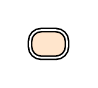
\begin{tikzpicture}[baseline={(0,-.1)}]
        \node[rectangle, line width=0.2mm, double, rounded corners, fill=orange!20,minimum size=1em,draw] at (0,0){$\ \ $};
    \end{tikzpicture}$ for one copy of the Auslander--Reiten quiver of $Q$}
        \label{fig:TiltA4}
    \end{figure}
\end{example}

The following result allows us to handle objects in $\Gen_\mathcal{E}(T)$ and those in $\Sub_\mathcal{E}(T)$ for $T \in \Tilt(\mathscr{A})$. See \cite{ASS06} for more details.

\begin{prop} \label{prop:GenSubT} Let $T \in \Tilt(\mathscr{A})$. The following assertions hold:
\begin{enumerate}[label=$(\roman*)$, itemsep=1mm]
    \item \label{GenET1} for any $M \in \Gen_\mathcal{E}(T)$, there exists a short $\mathcal{E}$-exact sequence \[\begin{tikzcd}
	 0 & T_1 & T_0 & M&  0.
	\arrow[from=1-1, to=1-2]
	\arrow[tail, from=1-2, to=1-3]
	\arrow[two heads,from=1-3, to=1-4]
	\arrow[from=1-4, to=1-5]
\end{tikzcd}\] where $T_0,T_1 \in \add(T)$; and,
\item \label{SubET1} for any $M \in \Sub_\mathcal{E}(T)$, there exists a short $\mathcal{E}$-exact sequence \[\begin{tikzcd}
	 0 & M & \Theta_0 &  \Theta_1 &  0.
	\arrow[from=1-1, to=1-2]
	\arrow[tail, from=1-2, to=1-3]
	\arrow[two heads,from=1-3, to=1-4]
	\arrow[from=1-4, to=1-5]
\end{tikzcd}\] where $\Theta_0,\Theta_1 \in \add(T)$.
\end{enumerate}   
\end{prop}

Before being further in the study of $\GS_\mathcal{E}(T)$ for any rigid object $T \in \mathscr{A}$, we can state a few noticeable results related to $\mathcal{E}$-adaptability.

\begin{lemma} \label{lem:TiltEadapt}
    For any rigid object $T \in \mathscr{A}$, the category $\add(T)$ is $\mathcal{E}$-adapted and closed under extension.
\end{lemma}

Thanks to what we proved previously, we have the following result.

\begin{cor} \label{cor:rigidEadapt}
    If $T \in \mathscr{A}$ is rigid, then $\GS_{\mathcal{E}}(T)$ is $\mathcal{E}$-adapted and closed under extension.
\end{cor}

\begin{proof}
     It follows from \cref{prop:Extclosed} and \cref{lem:TiltEadapt}.
\end{proof}

\begin{theorem}
\label{thm:maximal}
 Let $T \in \Tilt(\mathscr{A})$ be a tilting object. Then $\GS_\mathcal{E}(T)$ is a maximal $\mathcal{E}$-adapted subcategory of $\mathscr{A}$ closed under extensions which contains $T$.
\end{theorem}

\begin{proof}
Let $\mathscr{C} \subseteq \mathscr{A}$ be an $\mathcal{E}$-adapted subcategory closed under extensions that contains $T$. By \cref{conv:addsubcat}, to prove that $\mathscr{C} \subseteq \GS_\mathcal{E}(T)$, it is enough to show that all the objects in $\mathscr{C}$ are in $\GS_\mathcal{E}(T)$. 

Consider $V \in \mathscr{C}$. Suppose $V \in \proj(\mathscr{A})$. Since $T$ is tilting, by \cref{def:rigidtilting}, there is a short exact sequence 
\[\begin{tikzcd}
	\xi: & 0 & V & \Theta_0 & \Theta_1 &  0, & 
	\arrow[from=1-2, to=1-3]
	\arrow[tail, from=1-3, to=1-4]
	\arrow[two heads,from=1-4, to=1-5]
	\arrow[from=1-5, to=1-6]
\end{tikzcd}\] with $\Theta_0,\Theta_1 \in \add(T)$.
Since $V,\Theta_1 \in \mathscr{C}$ which is $\mathcal{E}$-adapted, then $\xi \in \mathcal{E}$. Thus $V \in \Sub_\mathcal{E}(T_0) \subseteq \GS_\mathcal{E}(T)$.

Assume that $V \notin \proj(\mathscr{A})$. Consider the projective resolution of $V$
\[\begin{tikzcd}
     0 & P_1 & P_0 & V &  0 & 
	\arrow[from=1-1, to=1-2]
	\arrow[tail, from=1-2, to=1-3]
	\arrow[two heads,from=1-3, to=1-4]
	\arrow[from=1-4, to=1-5]
\end{tikzcd}\] with $P_0,P_1 \in \proj(\mathscr{A})$. Since $T$ is tilting, by \cref{def:rigidtilting}, there is a short exact sequence
\[\begin{tikzcd}
   0 & P_1 & \Theta_0 & \Theta_1 &  0, & 
	\arrow[from=1-1, to=1-2]
	\arrow[tail,"\psi", from=1-2, to=1-3]
	\arrow[two heads,from=1-3, to=1-4]
	\arrow[from=1-4, to=1-5]
\end{tikzcd}\] with $\Theta_0,\Theta_1 \in \add(T)$. 
We obtain the following diagram by taking the pushout along $\psi$ and by using the cokernel lifting property.
\[\begin{tikzcd}
         & 0 & 0 & 0 &  \\
	0 & P_1 & P_0  & V &  0 \\
     0 & \Theta_0 & PO & V & 0 \\
      0 & \Theta_1 & C & 0 & 0 \\
       & 0 & 0 & 0 & 
	\arrow[from=2-1, to=2-2]
	\arrow[tail, from=2-2, to=2-3]
	\arrow[two heads,from=2-3, to=2-4]
	\arrow[from=2-4, to=2-5]
        \arrow[from=3-1, to=3-2]
	\arrow[tail, from=3-2, to=3-3]
	\arrow[two heads,from=3-3, to=3-4]
	\arrow[from=3-4, to=3-5]
        \arrow[from=4-1, to=4-2]
	\arrow[tail, from=4-2, to=4-3]
	\arrow[two heads,from=4-3, to=4-4]
	\arrow[from=4-4, to=4-5]
        \arrow[from=4-2, to=5-2]
	\arrow[two heads, from=3-2, to=4-2]
	\arrow[tail,"\psi",from=2-2, to=3-2]
	\arrow[from=1-2, to=2-2]
        \arrow[from=4-3, to=5-3]
	\arrow[two heads, from=3-3, to=4-3]
	\arrow[tail,from=2-3, to=3-3]
	\arrow[from=1-3, to=2-3]
        \arrow[from=4-4, to=5-4]
	\arrow[two heads, from=3-4, to=4-4]
	\arrow[equals,from=2-4, to=3-4]
	\arrow[from=1-4, to=2-4]
\end{tikzcd} \]
As the short sequences given by the three columns and those given by the first two rows of the above diagram are exact, by \cref{lem:3x3}, the short sequence given by the last row is exact too. So $C \cong \Theta_1$. Since $V,\Theta_0 \in \mathscr{C}$, by assumption on $\mathscr{C}$, then the middle row lies in $\mathcal{E}$, and $W = PO \in \mathscr{C}$.

Since $T$ is tilting, by \cref{def:rigidtilting}, there is also a short exact sequence 
\[\begin{tikzcd}
     0 & P_0 & \Theta_2 & \Theta_3 &  0, & 
	\arrow[from=1-1, to=1-2]
	\arrow[tail,"\phi", from=1-2, to=1-3]
	\arrow[two heads,from=1-3, to=1-4]
	\arrow[from=1-4, to=1-5]
\end{tikzcd}\] with $\Theta_2,\Theta_3 \in \add(T)$. Given the short exact sequence and the middle column of the diagram above, we obtain the following diagram by taking the pushout along $\phi$ and applying the cokernel lifting property again.
\[\begin{tikzcd}
         & 0 & 0 & 0 &  \\
	0 & P_0 & \Theta_2  & \Theta_3 &  0 \\
     0 & W & PO' & C' & 0 \\
      0 & \Theta_1 & \Theta_1 & 0 & 0 \\
       & 0 & 0 & 0 & 
	\arrow[from=2-1, to=2-2]
	\arrow[tail,"\phi", from=2-2, to=2-3]
	\arrow[two heads,from=2-3, to=2-4]
	\arrow[from=2-4, to=2-5]
        \arrow[from=3-1, to=3-2]
	\arrow[tail, from=3-2, to=3-3]
	\arrow[two heads,from=3-3, to=3-4]
	\arrow[from=3-4, to=3-5]
        \arrow[from=4-1, to=4-2]
	\arrow[equals, from=4-2, to=4-3]
	\arrow[two heads,from=4-3, to=4-4]
	\arrow[from=4-4, to=4-5]
        \arrow[from=4-2, to=5-2]
	\arrow[two heads, from=3-2, to=4-2]
	\arrow[tail,from=2-2, to=3-2]
	\arrow[from=1-2, to=2-2]
        \arrow[from=4-3, to=5-3]
	\arrow[two heads, from=3-3, to=4-3]
	\arrow[tail,from=2-3, to=3-3]
	\arrow[from=1-3, to=2-3]
        \arrow[from=4-4, to=5-4]
	\arrow[two heads, from=3-4, to=4-4]
	\arrow[from=2-4, to=3-4]
	\arrow[from=1-4, to=2-4]
\end{tikzcd} \]
As the short sequences given by the three rows and those given by the first two columns of the above diagram are exact, by \cref{lem:3x3}, the short sequence given by the last column is exact too. So $C' \cong \Theta_3$. Since $T$ is tilting, the middle column splits, hence $PO' \cong \Theta_1 \oplus \Theta_2$.

We get the following short exact sequence.
\[\begin{tikzcd}
    \varsigma: & 0 & W & \Theta_1 \oplus \Theta_2 & \Theta_3 &  0 & 
	\arrow[from=1-2, to=1-3]
	\arrow[tail, from=1-3, to=1-4]
	\arrow[two heads,from=1-4, to=1-5]
	\arrow[from=1-5, to=1-6]
\end{tikzcd}\]
As $W,\Theta_3 \in \mathscr{C}$, as $\mathscr{C}$ is $\mathcal{E}$-adapted, then $\varsigma \in \mathcal{E}$ and $W \in \Sub_\mathcal{E}(\Theta_1 \oplus \Theta_2) \subseteq \GS_\mathcal{E}(T)$.

We finally obtain the following short exact sequence from the middle row of the first diagram
\[\begin{tikzcd}
    \mu: & 0 & T_0 & W & V &  0 & 
	\arrow[from=1-2, to=1-3]
	\arrow[tail, from=1-3, to=1-4]
	\arrow[two heads,from=1-4, to=1-5]
	\arrow[from=1-5, to=1-6]
\end{tikzcd}\]
As $\mu \in \mathcal{E}$ and $W \in \GS_\mathcal{E}(T)$, we get that $V \in \Gen_\mathcal{E}(W) \subseteq \GS_\mathcal{E}(T)$. 

So all the objects in $\mathscr{C}$ are in $\GS_\mathcal{E}(T)$, and therefore, we get the desired result.
\end{proof}

Following the proof, the corollary below occurs.

\begin{cor} \label{cor:GS2=GSanduniqueESerre}
   Let $T \in \Tilt(\mathscr{A})$ be a tilting object. The following assertions hold:
   \begin{enumerate}[label=$(\alph*)$, itemsep=1mm]
       \item we have $\GS_\mathcal{E}(T) = \GS_\mathcal{E}^2(T)$, and moreover, if $T$ is an $\mathcal{E}$-projective object, then $\GS_\mathcal{E}(T) = \GS_\mathcal{E}^1(T)$; and,
       \item $\GS_\mathcal{E}(T)$ is the unique $\mathcal{E}$-adapted $\mathcal{E}$-Serre subcategory of $\mathscr{A}$ containing $T$.
   \end{enumerate}
\end{cor}

\begin{proof}
    The assertion $(a)$ follows directly from the proof of \cref{thm:maximal}. The assertion $(b)$ is a direct consequence of both \cref{thm:maximal} and \cref{cor:ESerre} $(d)$.
\end{proof}

Note that, in general, a maximal $\mathcal{E}$-adapted subcategory is not extension-closed. 


\begin{example} \label{ex:dontworkforanyE}
Consider $\mathscr{A} = \rep Q$ with
$Q = 1 \longrightarrow 2 \longrightarrow 3$. Fix the exact structure $\mathcal{E}'$ generated by the two following Auslander--Reiten sequences.
\[\begin{tikzcd}
    \xi_1: & 0 &  X_{\llrr{3}} & X_{\llrr{2,3}} & X_{\llrr{2}} & 0 
	\arrow[from=1-2, to=1-3]
	\arrow[tail, from=1-3, to=1-4]
	\arrow[two heads,from=1-4, to=1-5]
	\arrow[from=1-5, to=1-6]
\end{tikzcd}\]
\[\begin{tikzcd}
    \xi_2: & 0 &  X_{\llrr{2}} & X_{\llrr{1,2}} & X_{\llrr{1}} & 0 
	\arrow[from=1-2, to=1-3]
	\arrow[tail, from=1-3, to=1-4]
	\arrow[two heads,from=1-4, to=1-5]
	\arrow[from=1-5, to=1-6]
\end{tikzcd}\]

Let $\mathscr{C} = \add(X_{\llrr{1}}, X_{\llrr{2}}, X_{\llrr{3}}, X_{\llrr{1;3}})$ (see \cref{fig:NonExt-closed2}). We can check that $\mathscr{C}$ is a maximal $\mathcal{E}'$-adapted subcategory of $\mathscr{A}$, but $\mathscr{C}$ is not closed under extension.


\begin{figure}[!ht]
    \centering
    \begin{tikzpicture}[line width=.3mm, ->, >= angle 60]
		\node (23) at (1,-1){\scalebox{.9}{$\llrr{2,3}$}};
		\node[circle,line width=0.2mm,double,fill=lava!20,draw] (3) at (0,-2){\scalebox{.9}{$\llrr{3}$}};
		\node[circle,line width=0.2mm,double,fill=lava!20,draw] (13) at (2,0){\scalebox{.9}{$\llrr{1,3}$}};
		\node[circle,line width=0.2mm,double,fill=lava!20,draw] (2) at (2,-2){\scalebox{.9}{$\llrr{2}$}};
		\node (12) at (3,-1){\scalebox{.9}{$\llrr{1,2}$}};
		\node[circle,line width=0.2mm,double,fill=lava!20,draw] (1) at (4,-2){\scalebox{.9}{$\llrr{1}$}};
								
		\draw (3) -- (23);
		\draw (23) -- (13);
		\draw (23) -- (2);
		\draw (13) -- (12);
		\draw (2) -- (12);
		\draw (12) -- (1);
        \end{tikzpicture}
    \caption[fragile]{The Auslander--Reiten quiver of $Q$ in \cref{ex:Eadaptednonextclosed}. We have $\mathscr{C} = \add \left( \protect\begin{tikzpicture}[baseline={(0,-.1)}]
        \node[circle, line width=0.2mm, double, fill=lava!20,minimum size=1em,draw] at (0,0){$ $};
    \end{tikzpicture}\right) = \GS_{\mathcal{E}'}(\mathscr{C})$, and we can check that $\mathscr{C}$ is not closed under extensions even though it is a maximal $\mathcal{E}'$-adapted subcategory of $\mathscr{A}$.}
    \label{fig:NonExt-closed2}
\end{figure}           
\end{example}


